\documentclass[twoside]{book}

% Packages required by doxygen
\usepackage{fixltx2e}
\usepackage{calc}
\usepackage{doxygen}
\usepackage[export]{adjustbox} % also loads graphicx
\usepackage{graphicx}
\usepackage[utf8]{inputenc}
\usepackage{makeidx}
\usepackage{multicol}
\usepackage{multirow}
\PassOptionsToPackage{warn}{textcomp}
\usepackage{textcomp}
\usepackage[nointegrals]{wasysym}
\usepackage[table]{xcolor}

% Font selection
\usepackage[T1]{fontenc}
\usepackage[scaled=.90]{helvet}
\usepackage{courier}
\usepackage{amssymb}
\usepackage{sectsty}
\renewcommand{\familydefault}{\sfdefault}
\allsectionsfont{%
  \fontseries{bc}\selectfont%
  \color{darkgray}%
}
\renewcommand{\DoxyLabelFont}{%
  \fontseries{bc}\selectfont%
  \color{darkgray}%
}
\newcommand{\+}{\discretionary{\mbox{\scriptsize$\hookleftarrow$}}{}{}}

% Page & text layout
\usepackage{geometry}
\geometry{%
  a4paper,%
  top=2.5cm,%
  bottom=2.5cm,%
  left=2.5cm,%
  right=2.5cm%
}
\tolerance=750
\hfuzz=15pt
\hbadness=750
\setlength{\emergencystretch}{15pt}
\setlength{\parindent}{0cm}
\setlength{\parskip}{3ex plus 2ex minus 2ex}
\makeatletter
\renewcommand{\paragraph}{%
  \@startsection{paragraph}{4}{0ex}{-1.0ex}{1.0ex}{%
    \normalfont\normalsize\bfseries\SS@parafont%
  }%
}
\renewcommand{\subparagraph}{%
  \@startsection{subparagraph}{5}{0ex}{-1.0ex}{1.0ex}{%
    \normalfont\normalsize\bfseries\SS@subparafont%
  }%
}
\makeatother

% Headers & footers
\usepackage{fancyhdr}
\pagestyle{fancyplain}
\fancyhead[LE]{\fancyplain{}{\bfseries\thepage}}
\fancyhead[CE]{\fancyplain{}{}}
\fancyhead[RE]{\fancyplain{}{\bfseries\leftmark}}
\fancyhead[LO]{\fancyplain{}{\bfseries\rightmark}}
\fancyhead[CO]{\fancyplain{}{}}
\fancyhead[RO]{\fancyplain{}{\bfseries\thepage}}
\fancyfoot[LE]{\fancyplain{}{}}
\fancyfoot[CE]{\fancyplain{}{}}
\fancyfoot[RE]{\fancyplain{}{\bfseries\scriptsize Generated by Doxygen }}
\fancyfoot[LO]{\fancyplain{}{\bfseries\scriptsize Generated by Doxygen }}
\fancyfoot[CO]{\fancyplain{}{}}
\fancyfoot[RO]{\fancyplain{}{}}
\renewcommand{\footrulewidth}{0.4pt}
\renewcommand{\chaptermark}[1]{%
  \markboth{#1}{}%
}
\renewcommand{\sectionmark}[1]{%
  \markright{\thesection\ #1}%
}

% Indices & bibliography
\usepackage{natbib}
\usepackage[titles]{tocloft}
\setcounter{tocdepth}{3}
\setcounter{secnumdepth}{5}
\makeindex

% Hyperlinks (required, but should be loaded last)
\usepackage{ifpdf}
\ifpdf
  \usepackage[pdftex,pagebackref=true]{hyperref}
\else
  \usepackage[ps2pdf,pagebackref=true]{hyperref}
\fi
\hypersetup{%
  colorlinks=true,%
  linkcolor=blue,%
  citecolor=blue,%
  unicode%
}

% Custom commands
\newcommand{\clearemptydoublepage}{%
  \newpage{\pagestyle{empty}\cleardoublepage}%
}

\usepackage{caption}
\captionsetup{labelsep=space,justification=centering,font={bf},singlelinecheck=off,skip=4pt,position=top}

%===== C O N T E N T S =====

\begin{document}

% Titlepage & ToC
\hypersetup{pageanchor=false,
             bookmarksnumbered=true,
             pdfencoding=unicode
            }
\pagenumbering{alph}
\begin{titlepage}
\vspace*{7cm}
\begin{center}%
{\Large cpp\+\_\+javascript\+\_\+core }\\
\vspace*{1cm}
{\large Generated by Doxygen 1.8.14}\\
\end{center}
\end{titlepage}
\clearemptydoublepage
\pagenumbering{roman}
\tableofcontents
\clearemptydoublepage
\pagenumbering{arabic}
\hypersetup{pageanchor=true}

%--- Begin generated contents ---
\chapter{Namespace Index}
\section{Namespace List}
Here is a list of all namespaces with brief descriptions\+:\begin{DoxyCompactList}
\item\contentsline{section}{\mbox{\hyperlink{namespacecpp__javascriptcore}{cpp\+\_\+javascriptcore}} }{\pageref{namespacecpp__javascriptcore}}{}
\end{DoxyCompactList}

\chapter{Hierarchical Index}
\section{Class Hierarchy}
This inheritance list is sorted roughly, but not completely, alphabetically\+:\begin{DoxyCompactList}
\item \contentsline{section}{cpp\+\_\+javascriptcore\+:\+:C\+J\+S\+Class}{\pageref{classcpp__javascriptcore_1_1_c_j_s_class}}{}
\item \contentsline{section}{cpp\+\_\+javascriptcore\+:\+:C\+J\+S\+Constructor}{\pageref{classcpp__javascriptcore_1_1_c_j_s_constructor}}{}
\item \contentsline{section}{cpp\+\_\+javascriptcore\+:\+:C\+J\+S\+Context}{\pageref{classcpp__javascriptcore_1_1_c_j_s_context}}{}
\item \contentsline{section}{C\+J\+S\+Export\+Builder}{\pageref{class_c_j_s_export_builder}}{}
\item \contentsline{section}{cpp\+\_\+javascriptcore\+:\+:C\+J\+S\+Function}{\pageref{classcpp__javascriptcore_1_1_c_j_s_function}}{}
\item \contentsline{section}{cpp\+\_\+javascriptcore\+:\+:C\+J\+S\+Object}{\pageref{classcpp__javascriptcore_1_1_c_j_s_object}}{}
\item \contentsline{section}{cpp\+\_\+javascriptcore\+:\+:C\+J\+S\+Value}{\pageref{classcpp__javascriptcore_1_1_c_j_s_value}}{}
\item Component\begin{DoxyCompactList}
\item \contentsline{section}{Main\+Component}{\pageref{class_main_component}}{}
\end{DoxyCompactList}
\item Document\+Window\begin{DoxyCompactList}
\item \contentsline{section}{React\+Native\+J\+U\+C\+E\+Step1\+Application\+:\+:Main\+Window}{\pageref{class_react_native_j_u_c_e_step1_application_1_1_main_window}}{}
\end{DoxyCompactList}
\item J\+U\+C\+E\+Application\begin{DoxyCompactList}
\item \contentsline{section}{React\+Native\+J\+U\+C\+E\+Step1\+Application}{\pageref{class_react_native_j_u_c_e_step1_application}}{}
\end{DoxyCompactList}
\item \contentsline{section}{cpp\+\_\+javascriptcore\+:\+:Null\+Literal}{\pageref{structcpp__javascriptcore_1_1_null_literal}}{}
\item \contentsline{section}{cpp\+\_\+javascriptcore\+:\+:Undefined\+Literal}{\pageref{structcpp__javascriptcore_1_1_undefined_literal}}{}
\end{DoxyCompactList}

\chapter{Class Index}
\section{Class List}
Here are the classes, structs, unions and interfaces with brief descriptions\+:\begin{DoxyCompactList}
\item\contentsline{section}{\mbox{\hyperlink{classcpp__javascriptcore_1_1_c_j_s_class}{cpp\+\_\+javascriptcore\+::\+C\+J\+S\+Class}} }{\pageref{classcpp__javascriptcore_1_1_c_j_s_class}}{}
\item\contentsline{section}{\mbox{\hyperlink{classcpp__javascriptcore_1_1_c_j_s_constructor}{cpp\+\_\+javascriptcore\+::\+C\+J\+S\+Constructor}} }{\pageref{classcpp__javascriptcore_1_1_c_j_s_constructor}}{}
\item\contentsline{section}{\mbox{\hyperlink{classcpp__javascriptcore_1_1_c_j_s_context}{cpp\+\_\+javascriptcore\+::\+C\+J\+S\+Context}} }{\pageref{classcpp__javascriptcore_1_1_c_j_s_context}}{}
\item\contentsline{section}{\mbox{\hyperlink{class_c_j_s_export_builder}{C\+J\+S\+Export\+Builder}} }{\pageref{class_c_j_s_export_builder}}{}
\item\contentsline{section}{\mbox{\hyperlink{classcpp__javascriptcore_1_1_c_j_s_function}{cpp\+\_\+javascriptcore\+::\+C\+J\+S\+Function}} }{\pageref{classcpp__javascriptcore_1_1_c_j_s_function}}{}
\item\contentsline{section}{\mbox{\hyperlink{classcpp__javascriptcore_1_1_c_j_s_object}{cpp\+\_\+javascriptcore\+::\+C\+J\+S\+Object}} }{\pageref{classcpp__javascriptcore_1_1_c_j_s_object}}{}
\item\contentsline{section}{\mbox{\hyperlink{classcpp__javascriptcore_1_1_c_j_s_value}{cpp\+\_\+javascriptcore\+::\+C\+J\+S\+Value}} }{\pageref{classcpp__javascriptcore_1_1_c_j_s_value}}{}
\item\contentsline{section}{\mbox{\hyperlink{class_main_component}{Main\+Component}} }{\pageref{class_main_component}}{}
\item\contentsline{section}{\mbox{\hyperlink{class_react_native_j_u_c_e_step1_application_1_1_main_window}{React\+Native\+J\+U\+C\+E\+Step1\+Application\+::\+Main\+Window}} }{\pageref{class_react_native_j_u_c_e_step1_application_1_1_main_window}}{}
\item\contentsline{section}{\mbox{\hyperlink{structcpp__javascriptcore_1_1_null_literal}{cpp\+\_\+javascriptcore\+::\+Null\+Literal}} }{\pageref{structcpp__javascriptcore_1_1_null_literal}}{}
\item\contentsline{section}{\mbox{\hyperlink{class_react_native_j_u_c_e_step1_application}{React\+Native\+J\+U\+C\+E\+Step1\+Application}} }{\pageref{class_react_native_j_u_c_e_step1_application}}{}
\item\contentsline{section}{\mbox{\hyperlink{structcpp__javascriptcore_1_1_undefined_literal}{cpp\+\_\+javascriptcore\+::\+Undefined\+Literal}} }{\pageref{structcpp__javascriptcore_1_1_undefined_literal}}{}
\end{DoxyCompactList}

\chapter{File Index}
\section{File List}
Here is a list of all files with brief descriptions\+:\begin{DoxyCompactList}
\item\contentsline{section}{Source/\mbox{\hyperlink{_main_8cpp}{Main.\+cpp}} }{\pageref{_main_8cpp}}{}
\item\contentsline{section}{Source/\mbox{\hyperlink{_main_component_8cpp}{Main\+Component.\+cpp}} }{\pageref{_main_component_8cpp}}{}
\item\contentsline{section}{Source/\mbox{\hyperlink{_main_component_8h}{Main\+Component.\+h}} }{\pageref{_main_component_8h}}{}
\item\contentsline{section}{Source/\+Cpp-\/\+Java\+Script\+Core/\mbox{\hyperlink{_c_j_s_class_8h}{C\+J\+S\+Class.\+h}} }{\pageref{_c_j_s_class_8h}}{}
\item\contentsline{section}{Source/\+Cpp-\/\+Java\+Script\+Core/\mbox{\hyperlink{_c_j_s_constructor_8cpp}{C\+J\+S\+Constructor.\+cpp}} }{\pageref{_c_j_s_constructor_8cpp}}{}
\item\contentsline{section}{Source/\+Cpp-\/\+Java\+Script\+Core/\mbox{\hyperlink{_c_j_s_constructor_8h}{C\+J\+S\+Constructor.\+h}} }{\pageref{_c_j_s_constructor_8h}}{}
\item\contentsline{section}{Source/\+Cpp-\/\+Java\+Script\+Core/\mbox{\hyperlink{_c_j_s_export_class_8h}{C\+J\+S\+Export\+Class.\+h}} }{\pageref{_c_j_s_export_class_8h}}{}
\item\contentsline{section}{Source/\+Cpp-\/\+Java\+Script\+Core/\mbox{\hyperlink{_c_j_s_function_8cpp}{C\+J\+S\+Function.\+cpp}} }{\pageref{_c_j_s_function_8cpp}}{}
\item\contentsline{section}{Source/\+Cpp-\/\+Java\+Script\+Core/\mbox{\hyperlink{_c_j_s_function_8h}{C\+J\+S\+Function.\+h}} }{\pageref{_c_j_s_function_8h}}{}
\item\contentsline{section}{Source/\+Cpp-\/\+Java\+Script\+Core/\mbox{\hyperlink{_c_j_s_object_8cpp}{C\+J\+S\+Object.\+cpp}} }{\pageref{_c_j_s_object_8cpp}}{}
\item\contentsline{section}{Source/\+Cpp-\/\+Java\+Script\+Core/\mbox{\hyperlink{_c_j_s_object_8h}{C\+J\+S\+Object.\+h}} }{\pageref{_c_j_s_object_8h}}{}
\item\contentsline{section}{Source/\+Cpp-\/\+Java\+Script\+Core/\mbox{\hyperlink{_c_j_s_util_8cpp}{C\+J\+S\+Util.\+cpp}} }{\pageref{_c_j_s_util_8cpp}}{}
\item\contentsline{section}{Source/\+Cpp-\/\+Java\+Script\+Core/\mbox{\hyperlink{_c_j_s_util_8h}{C\+J\+S\+Util.\+h}} }{\pageref{_c_j_s_util_8h}}{}
\item\contentsline{section}{Source/\+Cpp-\/\+Java\+Script\+Core/\mbox{\hyperlink{_c_j_s_value_8cpp}{C\+J\+S\+Value.\+cpp}} }{\pageref{_c_j_s_value_8cpp}}{}
\item\contentsline{section}{Source/\+Cpp-\/\+Java\+Script\+Core/\mbox{\hyperlink{_c_j_s_value_8h}{C\+J\+S\+Value.\+h}} }{\pageref{_c_j_s_value_8h}}{}
\item\contentsline{section}{Source/\+Cpp-\/\+Java\+Script\+Core/\mbox{\hyperlink{_cpp-_java_script_core_8cpp}{Cpp-\/\+Java\+Script\+Core.\+cpp}} }{\pageref{_cpp-_java_script_core_8cpp}}{}
\item\contentsline{section}{Source/\+Cpp-\/\+Java\+Script\+Core/\mbox{\hyperlink{_cpp-_java_script_core_8h}{Cpp-\/\+Java\+Script\+Core.\+h}} }{\pageref{_cpp-_java_script_core_8h}}{}
\item\contentsline{section}{Source/\+Cpp-\/\+Java\+Script\+Core/\mbox{\hyperlink{_magic_conversion_8cpp}{Magic\+Conversion.\+cpp}} }{\pageref{_magic_conversion_8cpp}}{}
\item\contentsline{section}{Source/\+Cpp-\/\+Java\+Script\+Core/\mbox{\hyperlink{_magic_conversion_8h}{Magic\+Conversion.\+h}} }{\pageref{_magic_conversion_8h}}{}
\item\contentsline{section}{Source/\+J\+S\+C-\/\+J\+U\+C\+E/\mbox{\hyperlink{_j_s_c-_j_u_c_e_8cpp}{J\+S\+C-\/\+J\+U\+C\+E.\+cpp}} }{\pageref{_j_s_c-_j_u_c_e_8cpp}}{}
\item\contentsline{section}{Source/\+J\+S\+C-\/\+J\+U\+C\+E/\mbox{\hyperlink{_j_s_c-_j_u_c_e_8h}{J\+S\+C-\/\+J\+U\+C\+E.\+h}} }{\pageref{_j_s_c-_j_u_c_e_8h}}{}
\end{DoxyCompactList}

\chapter{Namespace Documentation}
\hypertarget{namespacecpp__javascriptcore}{}\section{cpp\+\_\+javascriptcore Namespace Reference}
\label{namespacecpp__javascriptcore}\index{cpp\+\_\+javascriptcore@{cpp\+\_\+javascriptcore}}
\subsection*{Classes}
\begin{DoxyCompactItemize}
\item 
class \mbox{\hyperlink{classcpp__javascriptcore_1_1_c_j_s_class}{C\+J\+S\+Class}}
\item 
class \mbox{\hyperlink{classcpp__javascriptcore_1_1_c_j_s_constructor}{C\+J\+S\+Constructor}}
\item 
class \mbox{\hyperlink{classcpp__javascriptcore_1_1_c_j_s_context}{C\+J\+S\+Context}}
\item 
class \mbox{\hyperlink{classcpp__javascriptcore_1_1_c_j_s_function}{C\+J\+S\+Function}}
\item 
class \mbox{\hyperlink{classcpp__javascriptcore_1_1_c_j_s_object}{C\+J\+S\+Object}}
\item 
class \mbox{\hyperlink{classcpp__javascriptcore_1_1_c_j_s_value}{C\+J\+S\+Value}}
\item 
struct \mbox{\hyperlink{structcpp__javascriptcore_1_1_null_literal}{Null\+Literal}}
\item 
struct \mbox{\hyperlink{structcpp__javascriptcore_1_1_undefined_literal}{Undefined\+Literal}}
\end{DoxyCompactItemize}
\subsection*{Typedefs}
\begin{DoxyCompactItemize}
\item 
using \mbox{\hyperlink{namespacecpp__javascriptcore_ade392e059225cd35b14b1b7efb9d5a5b}{Cb\+J\+S\+Args\+Returning\+J\+S\+Value\+With\+Context}} = std\+::function$<$ J\+S\+Value\+Ref(J\+S\+Context\+Ref, J\+S\+Object\+Ref, size\+\_\+t, const J\+S\+Value\+Ref\mbox{[}$\,$\mbox{]})$>$
\end{DoxyCompactItemize}
\subsection*{Functions}
\begin{DoxyCompactItemize}
\item 
J\+S\+String\+Ref \mbox{\hyperlink{namespacecpp__javascriptcore_a64c0a5a8f178db673f0eb7704ee78816}{get\+J\+S\+String\+Ref\+From\+String}} (const std\+::string \&str)
\item 
std\+::vector$<$ J\+S\+Value\+Ref $>$ \mbox{\hyperlink{namespacecpp__javascriptcore_a5d52cd145305a6c024858e80973867e5}{convert\+Values}} (J\+S\+Context\+Ref context)
\item 
{\footnotesize template$<$typename Arg $>$ }\\\mbox{\hyperlink{classcpp__javascriptcore_1_1_c_j_s_value}{C\+J\+S\+Value}} \mbox{\hyperlink{namespacecpp__javascriptcore_a2ae1cd64b14aa12f56f503463a3dede6}{convert\+Value}} (J\+S\+Context\+Ref context, Arg value)
\item 
{\footnotesize template$<$typename Arg , typename... Args$>$ }\\std\+::vector$<$ J\+S\+Value\+Ref $>$ \mbox{\hyperlink{namespacecpp__javascriptcore_ad53bb2850a23b75e56b6d953fc90b552}{convert\+Values}} (J\+S\+Context\+Ref context, Arg value, Args... tail)
\item 
{\footnotesize template$<$typename Ret $>$ }\\Ret \mbox{\hyperlink{namespacecpp__javascriptcore_a63b8017b1766288a57631889bd4d205c}{from\+JS}} (J\+S\+Context\+Ref context, J\+S\+Value\+Ref value)
\item 
{\footnotesize template$<$typename F , typename Arg\+Types , std\+::size\+\_\+t N, std\+::size\+\_\+t... Idx$>$ }\\decltype(auto) \mbox{\hyperlink{namespacecpp__javascriptcore_a2c32796cd818b3a75a7dc6f033b4a596}{apply\+Impl}} (F fn, Arg\+Types \&args, std\+::index\+\_\+sequence$<$ Idx... $>$)
\item 
{\footnotesize template$<$typename F , typename Arg\+Types , std\+::size\+\_\+t N$>$ }\\decltype(auto) \mbox{\hyperlink{namespacecpp__javascriptcore_ae99580d5a07367766396914230c5cb4a}{apply}} (F fn, Arg\+Types \&args)
\item 
{\footnotesize template$<$typename Fn $>$ }\\\mbox{\hyperlink{classcpp__javascriptcore_1_1_c_j_s_function_a3cf83c4e33bfeafbe770047bb75556f5}{C\+J\+S\+Function\+::\+Callback}} \mbox{\hyperlink{namespacecpp__javascriptcore_ac75c77a83b4f02ba3e0529799f49a313}{make\+Callback}} (Fn \&\&callback)
\end{DoxyCompactItemize}


\subsection{Typedef Documentation}
\mbox{\Hypertarget{namespacecpp__javascriptcore_ade392e059225cd35b14b1b7efb9d5a5b}\label{namespacecpp__javascriptcore_ade392e059225cd35b14b1b7efb9d5a5b}} 
\index{cpp\+\_\+javascriptcore@{cpp\+\_\+javascriptcore}!Cb\+J\+S\+Args\+Returning\+J\+S\+Value\+With\+Context@{Cb\+J\+S\+Args\+Returning\+J\+S\+Value\+With\+Context}}
\index{Cb\+J\+S\+Args\+Returning\+J\+S\+Value\+With\+Context@{Cb\+J\+S\+Args\+Returning\+J\+S\+Value\+With\+Context}!cpp\+\_\+javascriptcore@{cpp\+\_\+javascriptcore}}
\subsubsection{\texorpdfstring{Cb\+J\+S\+Args\+Returning\+J\+S\+Value\+With\+Context}{CbJSArgsReturningJSValueWithContext}}
{\footnotesize\ttfamily using \mbox{\hyperlink{namespacecpp__javascriptcore_ade392e059225cd35b14b1b7efb9d5a5b}{cpp\+\_\+javascriptcore\+::\+Cb\+J\+S\+Args\+Returning\+J\+S\+Value\+With\+Context}} = typedef std\+::function$<$J\+S\+Value\+Ref (J\+S\+Context\+Ref, J\+S\+Object\+Ref, size\+\_\+t, const J\+S\+Value\+Ref\mbox{[}$\,$\mbox{]})$>$}



Definition at line 17 of file C\+J\+S\+Function.\+h.



\subsection{Function Documentation}
\mbox{\Hypertarget{namespacecpp__javascriptcore_ae99580d5a07367766396914230c5cb4a}\label{namespacecpp__javascriptcore_ae99580d5a07367766396914230c5cb4a}} 
\index{cpp\+\_\+javascriptcore@{cpp\+\_\+javascriptcore}!apply@{apply}}
\index{apply@{apply}!cpp\+\_\+javascriptcore@{cpp\+\_\+javascriptcore}}
\subsubsection{\texorpdfstring{apply()}{apply()}}
{\footnotesize\ttfamily template$<$typename F , typename Arg\+Types , std\+::size\+\_\+t N$>$ \\
decltype(auto) cpp\+\_\+javascriptcore\+::apply (\begin{DoxyParamCaption}\item[{F}]{fn,  }\item[{Arg\+Types \&}]{args }\end{DoxyParamCaption})}



Definition at line 41 of file Magic\+Conversion.\+h.

\mbox{\Hypertarget{namespacecpp__javascriptcore_a2c32796cd818b3a75a7dc6f033b4a596}\label{namespacecpp__javascriptcore_a2c32796cd818b3a75a7dc6f033b4a596}} 
\index{cpp\+\_\+javascriptcore@{cpp\+\_\+javascriptcore}!apply\+Impl@{apply\+Impl}}
\index{apply\+Impl@{apply\+Impl}!cpp\+\_\+javascriptcore@{cpp\+\_\+javascriptcore}}
\subsubsection{\texorpdfstring{apply\+Impl()}{applyImpl()}}
{\footnotesize\ttfamily template$<$typename F , typename Arg\+Types , std\+::size\+\_\+t N, std\+::size\+\_\+t... Idx$>$ \\
decltype(auto) cpp\+\_\+javascriptcore\+::apply\+Impl (\begin{DoxyParamCaption}\item[{F}]{fn,  }\item[{Arg\+Types \&}]{args,  }\item[{std\+::index\+\_\+sequence$<$ Idx... $>$}]{ }\end{DoxyParamCaption})}



Definition at line 36 of file Magic\+Conversion.\+h.

\mbox{\Hypertarget{namespacecpp__javascriptcore_a2ae1cd64b14aa12f56f503463a3dede6}\label{namespacecpp__javascriptcore_a2ae1cd64b14aa12f56f503463a3dede6}} 
\index{cpp\+\_\+javascriptcore@{cpp\+\_\+javascriptcore}!convert\+Value@{convert\+Value}}
\index{convert\+Value@{convert\+Value}!cpp\+\_\+javascriptcore@{cpp\+\_\+javascriptcore}}
\subsubsection{\texorpdfstring{convert\+Value()}{convertValue()}}
{\footnotesize\ttfamily template$<$typename Arg $>$ \\
\mbox{\hyperlink{classcpp__javascriptcore_1_1_c_j_s_value}{C\+J\+S\+Value}} cpp\+\_\+javascriptcore\+::convert\+Value (\begin{DoxyParamCaption}\item[{J\+S\+Context\+Ref}]{context,  }\item[{Arg}]{value }\end{DoxyParamCaption})}



Definition at line 13 of file Magic\+Conversion.\+h.

\mbox{\Hypertarget{namespacecpp__javascriptcore_a5d52cd145305a6c024858e80973867e5}\label{namespacecpp__javascriptcore_a5d52cd145305a6c024858e80973867e5}} 
\index{cpp\+\_\+javascriptcore@{cpp\+\_\+javascriptcore}!convert\+Values@{convert\+Values}}
\index{convert\+Values@{convert\+Values}!cpp\+\_\+javascriptcore@{cpp\+\_\+javascriptcore}}
\subsubsection{\texorpdfstring{convert\+Values()}{convertValues()}\hspace{0.1cm}{\footnotesize\ttfamily [1/2]}}
{\footnotesize\ttfamily std\+::vector$<$ J\+S\+Value\+Ref $>$ cpp\+\_\+javascriptcore\+::convert\+Values (\begin{DoxyParamCaption}\item[{J\+S\+Context\+Ref}]{context }\end{DoxyParamCaption})}



Definition at line 6 of file Magic\+Conversion.\+cpp.

\mbox{\Hypertarget{namespacecpp__javascriptcore_ad53bb2850a23b75e56b6d953fc90b552}\label{namespacecpp__javascriptcore_ad53bb2850a23b75e56b6d953fc90b552}} 
\index{cpp\+\_\+javascriptcore@{cpp\+\_\+javascriptcore}!convert\+Values@{convert\+Values}}
\index{convert\+Values@{convert\+Values}!cpp\+\_\+javascriptcore@{cpp\+\_\+javascriptcore}}
\subsubsection{\texorpdfstring{convert\+Values()}{convertValues()}\hspace{0.1cm}{\footnotesize\ttfamily [2/2]}}
{\footnotesize\ttfamily template$<$typename Arg , typename... Args$>$ \\
std\+::vector$<$J\+S\+Value\+Ref$>$ cpp\+\_\+javascriptcore\+::convert\+Values (\begin{DoxyParamCaption}\item[{J\+S\+Context\+Ref}]{context,  }\item[{Arg}]{value,  }\item[{Args...}]{tail }\end{DoxyParamCaption})}



Definition at line 21 of file Magic\+Conversion.\+h.

\mbox{\Hypertarget{namespacecpp__javascriptcore_a63b8017b1766288a57631889bd4d205c}\label{namespacecpp__javascriptcore_a63b8017b1766288a57631889bd4d205c}} 
\index{cpp\+\_\+javascriptcore@{cpp\+\_\+javascriptcore}!from\+JS@{from\+JS}}
\index{from\+JS@{from\+JS}!cpp\+\_\+javascriptcore@{cpp\+\_\+javascriptcore}}
\subsubsection{\texorpdfstring{from\+J\+S()}{fromJS()}}
{\footnotesize\ttfamily template$<$typename Ret $>$ \\
Ret cpp\+\_\+javascriptcore\+::from\+JS (\begin{DoxyParamCaption}\item[{J\+S\+Context\+Ref}]{context,  }\item[{J\+S\+Value\+Ref}]{value }\end{DoxyParamCaption})}



Definition at line 29 of file Magic\+Conversion.\+h.

\mbox{\Hypertarget{namespacecpp__javascriptcore_a64c0a5a8f178db673f0eb7704ee78816}\label{namespacecpp__javascriptcore_a64c0a5a8f178db673f0eb7704ee78816}} 
\index{cpp\+\_\+javascriptcore@{cpp\+\_\+javascriptcore}!get\+J\+S\+String\+Ref\+From\+String@{get\+J\+S\+String\+Ref\+From\+String}}
\index{get\+J\+S\+String\+Ref\+From\+String@{get\+J\+S\+String\+Ref\+From\+String}!cpp\+\_\+javascriptcore@{cpp\+\_\+javascriptcore}}
\subsubsection{\texorpdfstring{get\+J\+S\+String\+Ref\+From\+String()}{getJSStringRefFromString()}}
{\footnotesize\ttfamily J\+S\+String\+Ref cpp\+\_\+javascriptcore\+::get\+J\+S\+String\+Ref\+From\+String (\begin{DoxyParamCaption}\item[{const std\+::string \&}]{str }\end{DoxyParamCaption})}



Definition at line 6 of file C\+J\+S\+Util.\+cpp.

\mbox{\Hypertarget{namespacecpp__javascriptcore_ac75c77a83b4f02ba3e0529799f49a313}\label{namespacecpp__javascriptcore_ac75c77a83b4f02ba3e0529799f49a313}} 
\index{cpp\+\_\+javascriptcore@{cpp\+\_\+javascriptcore}!make\+Callback@{make\+Callback}}
\index{make\+Callback@{make\+Callback}!cpp\+\_\+javascriptcore@{cpp\+\_\+javascriptcore}}
\subsubsection{\texorpdfstring{make\+Callback()}{makeCallback()}}
{\footnotesize\ttfamily template$<$typename Fn $>$ \\
\mbox{\hyperlink{classcpp__javascriptcore_1_1_c_j_s_function_a3cf83c4e33bfeafbe770047bb75556f5}{C\+J\+S\+Function\+::\+Callback}} cpp\+\_\+javascriptcore\+::make\+Callback (\begin{DoxyParamCaption}\item[{Fn \&\&}]{callback }\end{DoxyParamCaption})}



Definition at line 46 of file Magic\+Conversion.\+h.


\chapter{Class Documentation}
\hypertarget{classcpp__javascriptcore_1_1_c_j_s_class}{}\section{cpp\+\_\+javascriptcore\+:\+:C\+J\+S\+Class Class Reference}
\label{classcpp__javascriptcore_1_1_c_j_s_class}\index{cpp\+\_\+javascriptcore\+::\+C\+J\+S\+Class@{cpp\+\_\+javascriptcore\+::\+C\+J\+S\+Class}}


{\ttfamily \#include $<$C\+J\+S\+Class.\+h$>$}

\subsection*{Public Member Functions}
\begin{DoxyCompactItemize}
\item 
\mbox{\hyperlink{classcpp__javascriptcore_1_1_c_j_s_class_ae2c13d7518c778746bfbedbaf650a24c}{C\+J\+S\+Class}} (J\+S\+Class\+Ref klass\+\_\+)
\item 
\mbox{\hyperlink{classcpp__javascriptcore_1_1_c_j_s_class_a24e99d07c375b6bbc30abbea7a8a528b}{$\sim$\+C\+J\+S\+Class}} ()
\item 
J\+S\+Class\+Ref \mbox{\hyperlink{classcpp__javascriptcore_1_1_c_j_s_class_acb05238883927560fa7e43001226bc91}{get\+Class}} ()
\end{DoxyCompactItemize}


\subsection{Detailed Description}


Definition at line 10 of file C\+J\+S\+Class.\+h.



\subsection{Constructor \& Destructor Documentation}
\mbox{\Hypertarget{classcpp__javascriptcore_1_1_c_j_s_class_ae2c13d7518c778746bfbedbaf650a24c}\label{classcpp__javascriptcore_1_1_c_j_s_class_ae2c13d7518c778746bfbedbaf650a24c}} 
\index{cpp\+\_\+javascriptcore\+::\+C\+J\+S\+Class@{cpp\+\_\+javascriptcore\+::\+C\+J\+S\+Class}!C\+J\+S\+Class@{C\+J\+S\+Class}}
\index{C\+J\+S\+Class@{C\+J\+S\+Class}!cpp\+\_\+javascriptcore\+::\+C\+J\+S\+Class@{cpp\+\_\+javascriptcore\+::\+C\+J\+S\+Class}}
\subsubsection{\texorpdfstring{C\+J\+S\+Class()}{CJSClass()}}
{\footnotesize\ttfamily cpp\+\_\+javascriptcore\+::\+C\+J\+S\+Class\+::\+C\+J\+S\+Class (\begin{DoxyParamCaption}\item[{J\+S\+Class\+Ref}]{klass\+\_\+ }\end{DoxyParamCaption})\hspace{0.3cm}{\ttfamily [inline]}}



Definition at line 13 of file C\+J\+S\+Class.\+h.

\mbox{\Hypertarget{classcpp__javascriptcore_1_1_c_j_s_class_a24e99d07c375b6bbc30abbea7a8a528b}\label{classcpp__javascriptcore_1_1_c_j_s_class_a24e99d07c375b6bbc30abbea7a8a528b}} 
\index{cpp\+\_\+javascriptcore\+::\+C\+J\+S\+Class@{cpp\+\_\+javascriptcore\+::\+C\+J\+S\+Class}!````~C\+J\+S\+Class@{$\sim$\+C\+J\+S\+Class}}
\index{````~C\+J\+S\+Class@{$\sim$\+C\+J\+S\+Class}!cpp\+\_\+javascriptcore\+::\+C\+J\+S\+Class@{cpp\+\_\+javascriptcore\+::\+C\+J\+S\+Class}}
\subsubsection{\texorpdfstring{$\sim$\+C\+J\+S\+Class()}{~CJSClass()}}
{\footnotesize\ttfamily cpp\+\_\+javascriptcore\+::\+C\+J\+S\+Class\+::$\sim$\+C\+J\+S\+Class (\begin{DoxyParamCaption}{ }\end{DoxyParamCaption})\hspace{0.3cm}{\ttfamily [inline]}}



Definition at line 17 of file C\+J\+S\+Class.\+h.



\subsection{Member Function Documentation}
\mbox{\Hypertarget{classcpp__javascriptcore_1_1_c_j_s_class_acb05238883927560fa7e43001226bc91}\label{classcpp__javascriptcore_1_1_c_j_s_class_acb05238883927560fa7e43001226bc91}} 
\index{cpp\+\_\+javascriptcore\+::\+C\+J\+S\+Class@{cpp\+\_\+javascriptcore\+::\+C\+J\+S\+Class}!get\+Class@{get\+Class}}
\index{get\+Class@{get\+Class}!cpp\+\_\+javascriptcore\+::\+C\+J\+S\+Class@{cpp\+\_\+javascriptcore\+::\+C\+J\+S\+Class}}
\subsubsection{\texorpdfstring{get\+Class()}{getClass()}}
{\footnotesize\ttfamily J\+S\+Class\+Ref cpp\+\_\+javascriptcore\+::\+C\+J\+S\+Class\+::get\+Class (\begin{DoxyParamCaption}{ }\end{DoxyParamCaption})\hspace{0.3cm}{\ttfamily [inline]}}



Definition at line 21 of file C\+J\+S\+Class.\+h.



The documentation for this class was generated from the following file\+:\begin{DoxyCompactItemize}
\item 
Source/\+Cpp-\/\+Java\+Script\+Core/\mbox{\hyperlink{_c_j_s_class_8h}{C\+J\+S\+Class.\+h}}\end{DoxyCompactItemize}

\hypertarget{classcpp__javascriptcore_1_1_c_j_s_constructor}{}\section{cpp\+\_\+javascriptcore\+:\+:C\+J\+S\+Constructor Class Reference}
\label{classcpp__javascriptcore_1_1_c_j_s_constructor}\index{cpp\+\_\+javascriptcore\+::\+C\+J\+S\+Constructor@{cpp\+\_\+javascriptcore\+::\+C\+J\+S\+Constructor}}


{\ttfamily \#include $<$C\+J\+S\+Constructor.\+h$>$}

\subsection*{Public Types}
\begin{DoxyCompactItemize}
\item 
using \mbox{\hyperlink{classcpp__javascriptcore_1_1_c_j_s_constructor_aeeebb95fa01f05a9f0793ed7b176e759}{Constructor}} = std\+::function$<$ J\+S\+Object\+Ref(J\+S\+Context\+Ref, J\+S\+Object\+Ref, size\+\_\+t, const J\+S\+Value\+Ref\mbox{[}$\,$\mbox{]}, J\+S\+Value\+Ref $\ast$)$>$
\end{DoxyCompactItemize}
\subsection*{Public Member Functions}
\begin{DoxyCompactItemize}
\item 
\mbox{\hyperlink{classcpp__javascriptcore_1_1_c_j_s_constructor_aa7487dce0f60a47ace1056f8218d2128}{C\+J\+S\+Constructor}} (J\+S\+Context\+Ref context\+\_\+, J\+S\+Class\+Ref klass\+\_\+, \mbox{\hyperlink{classcpp__javascriptcore_1_1_c_j_s_constructor_aeeebb95fa01f05a9f0793ed7b176e759}{Constructor}} \&constructor)
\item 
\mbox{\hyperlink{classcpp__javascriptcore_1_1_c_j_s_constructor_aba23ba6a23a67ab76adb851536ac5394}{$\sim$\+C\+J\+S\+Constructor}} ()
\item 
J\+S\+Class\+Ref \mbox{\hyperlink{classcpp__javascriptcore_1_1_c_j_s_constructor_a3ad524ec0305f3709842e451fc7c684c}{get\+Class}} ()
\item 
J\+S\+Object\+Ref \mbox{\hyperlink{classcpp__javascriptcore_1_1_c_j_s_constructor_ad2fabad070c8a98d05c56bbc83f0705a}{get\+Constructor}} ()
\end{DoxyCompactItemize}


\subsection{Detailed Description}


Definition at line 10 of file C\+J\+S\+Constructor.\+h.



\subsection{Member Typedef Documentation}
\mbox{\Hypertarget{classcpp__javascriptcore_1_1_c_j_s_constructor_aeeebb95fa01f05a9f0793ed7b176e759}\label{classcpp__javascriptcore_1_1_c_j_s_constructor_aeeebb95fa01f05a9f0793ed7b176e759}} 
\index{cpp\+\_\+javascriptcore\+::\+C\+J\+S\+Constructor@{cpp\+\_\+javascriptcore\+::\+C\+J\+S\+Constructor}!Constructor@{Constructor}}
\index{Constructor@{Constructor}!cpp\+\_\+javascriptcore\+::\+C\+J\+S\+Constructor@{cpp\+\_\+javascriptcore\+::\+C\+J\+S\+Constructor}}
\subsubsection{\texorpdfstring{Constructor}{Constructor}}
{\footnotesize\ttfamily using \mbox{\hyperlink{classcpp__javascriptcore_1_1_c_j_s_constructor_aeeebb95fa01f05a9f0793ed7b176e759}{cpp\+\_\+javascriptcore\+::\+C\+J\+S\+Constructor\+::\+Constructor}} =  std\+::function$<$J\+S\+Object\+Ref (J\+S\+Context\+Ref, J\+S\+Object\+Ref, size\+\_\+t, const J\+S\+Value\+Ref\mbox{[}$\,$\mbox{]}, J\+S\+Value\+Ref$\ast$)$>$}



Definition at line 13 of file C\+J\+S\+Constructor.\+h.



\subsection{Constructor \& Destructor Documentation}
\mbox{\Hypertarget{classcpp__javascriptcore_1_1_c_j_s_constructor_aa7487dce0f60a47ace1056f8218d2128}\label{classcpp__javascriptcore_1_1_c_j_s_constructor_aa7487dce0f60a47ace1056f8218d2128}} 
\index{cpp\+\_\+javascriptcore\+::\+C\+J\+S\+Constructor@{cpp\+\_\+javascriptcore\+::\+C\+J\+S\+Constructor}!C\+J\+S\+Constructor@{C\+J\+S\+Constructor}}
\index{C\+J\+S\+Constructor@{C\+J\+S\+Constructor}!cpp\+\_\+javascriptcore\+::\+C\+J\+S\+Constructor@{cpp\+\_\+javascriptcore\+::\+C\+J\+S\+Constructor}}
\subsubsection{\texorpdfstring{C\+J\+S\+Constructor()}{CJSConstructor()}}
{\footnotesize\ttfamily cpp\+\_\+javascriptcore\+::\+C\+J\+S\+Constructor\+::\+C\+J\+S\+Constructor (\begin{DoxyParamCaption}\item[{J\+S\+Context\+Ref}]{context\+\_\+,  }\item[{J\+S\+Class\+Ref}]{klass\+\_\+,  }\item[{\mbox{\hyperlink{classcpp__javascriptcore_1_1_c_j_s_constructor_aeeebb95fa01f05a9f0793ed7b176e759}{Constructor}} \&}]{constructor }\end{DoxyParamCaption})}



Definition at line 6 of file C\+J\+S\+Constructor.\+cpp.

\mbox{\Hypertarget{classcpp__javascriptcore_1_1_c_j_s_constructor_aba23ba6a23a67ab76adb851536ac5394}\label{classcpp__javascriptcore_1_1_c_j_s_constructor_aba23ba6a23a67ab76adb851536ac5394}} 
\index{cpp\+\_\+javascriptcore\+::\+C\+J\+S\+Constructor@{cpp\+\_\+javascriptcore\+::\+C\+J\+S\+Constructor}!````~C\+J\+S\+Constructor@{$\sim$\+C\+J\+S\+Constructor}}
\index{````~C\+J\+S\+Constructor@{$\sim$\+C\+J\+S\+Constructor}!cpp\+\_\+javascriptcore\+::\+C\+J\+S\+Constructor@{cpp\+\_\+javascriptcore\+::\+C\+J\+S\+Constructor}}
\subsubsection{\texorpdfstring{$\sim$\+C\+J\+S\+Constructor()}{~CJSConstructor()}}
{\footnotesize\ttfamily cpp\+\_\+javascriptcore\+::\+C\+J\+S\+Constructor\+::$\sim$\+C\+J\+S\+Constructor (\begin{DoxyParamCaption}{ }\end{DoxyParamCaption})}



Definition at line 12 of file C\+J\+S\+Constructor.\+cpp.



\subsection{Member Function Documentation}
\mbox{\Hypertarget{classcpp__javascriptcore_1_1_c_j_s_constructor_a3ad524ec0305f3709842e451fc7c684c}\label{classcpp__javascriptcore_1_1_c_j_s_constructor_a3ad524ec0305f3709842e451fc7c684c}} 
\index{cpp\+\_\+javascriptcore\+::\+C\+J\+S\+Constructor@{cpp\+\_\+javascriptcore\+::\+C\+J\+S\+Constructor}!get\+Class@{get\+Class}}
\index{get\+Class@{get\+Class}!cpp\+\_\+javascriptcore\+::\+C\+J\+S\+Constructor@{cpp\+\_\+javascriptcore\+::\+C\+J\+S\+Constructor}}
\subsubsection{\texorpdfstring{get\+Class()}{getClass()}}
{\footnotesize\ttfamily J\+S\+Class\+Ref cpp\+\_\+javascriptcore\+::\+C\+J\+S\+Constructor\+::get\+Class (\begin{DoxyParamCaption}{ }\end{DoxyParamCaption})\hspace{0.3cm}{\ttfamily [inline]}}



Definition at line 29 of file C\+J\+S\+Constructor.\+h.

\mbox{\Hypertarget{classcpp__javascriptcore_1_1_c_j_s_constructor_ad2fabad070c8a98d05c56bbc83f0705a}\label{classcpp__javascriptcore_1_1_c_j_s_constructor_ad2fabad070c8a98d05c56bbc83f0705a}} 
\index{cpp\+\_\+javascriptcore\+::\+C\+J\+S\+Constructor@{cpp\+\_\+javascriptcore\+::\+C\+J\+S\+Constructor}!get\+Constructor@{get\+Constructor}}
\index{get\+Constructor@{get\+Constructor}!cpp\+\_\+javascriptcore\+::\+C\+J\+S\+Constructor@{cpp\+\_\+javascriptcore\+::\+C\+J\+S\+Constructor}}
\subsubsection{\texorpdfstring{get\+Constructor()}{getConstructor()}}
{\footnotesize\ttfamily J\+S\+Object\+Ref cpp\+\_\+javascriptcore\+::\+C\+J\+S\+Constructor\+::get\+Constructor (\begin{DoxyParamCaption}{ }\end{DoxyParamCaption})\hspace{0.3cm}{\ttfamily [inline]}}



Definition at line 34 of file C\+J\+S\+Constructor.\+h.



The documentation for this class was generated from the following files\+:\begin{DoxyCompactItemize}
\item 
Source/\+Cpp-\/\+Java\+Script\+Core/\mbox{\hyperlink{_c_j_s_constructor_8h}{C\+J\+S\+Constructor.\+h}}\item 
Source/\+Cpp-\/\+Java\+Script\+Core/\mbox{\hyperlink{_c_j_s_constructor_8cpp}{C\+J\+S\+Constructor.\+cpp}}\end{DoxyCompactItemize}

\hypertarget{classcpp__javascriptcore_1_1_c_j_s_context}{}\section{cpp\+\_\+javascriptcore\+:\+:C\+J\+S\+Context Class Reference}
\label{classcpp__javascriptcore_1_1_c_j_s_context}\index{cpp\+\_\+javascriptcore\+::\+C\+J\+S\+Context@{cpp\+\_\+javascriptcore\+::\+C\+J\+S\+Context}}


{\ttfamily \#include $<$Cpp-\/\+Java\+Script\+Core.\+h$>$}

\subsection*{Public Member Functions}
\begin{DoxyCompactItemize}
\item 
\mbox{\hyperlink{classcpp__javascriptcore_1_1_c_j_s_context_a2bb3c165dca01f4b7de91c5512d59d9e}{C\+J\+S\+Context}} ()
\item 
\mbox{\hyperlink{classcpp__javascriptcore_1_1_c_j_s_context_a5085045b6def320b1719e20b33987669}{$\sim$\+C\+J\+S\+Context}} ()
\item 
Either$<$ \mbox{\hyperlink{classcpp__javascriptcore_1_1_c_j_s_value}{C\+J\+S\+Value}}, std\+::string $>$ \mbox{\hyperlink{classcpp__javascriptcore_1_1_c_j_s_context_abe49a3875a40cb94e5e5249be7a91a9b}{evaluate\+Script}} (const std\+::string \&script)
\item 
\mbox{\hyperlink{classcpp__javascriptcore_1_1_c_j_s_object}{C\+J\+S\+Object}} \mbox{\hyperlink{classcpp__javascriptcore_1_1_c_j_s_context_a35e34df7a2ff0bcda8ef35d43947fa58}{get\+Global\+Object}} ()
\item 
J\+S\+Global\+Context\+Ref \mbox{\hyperlink{classcpp__javascriptcore_1_1_c_j_s_context_a2196952e270dc02a646febe5f054545b}{get\+Context}} ()
\item 
\mbox{\hyperlink{classcpp__javascriptcore_1_1_c_j_s_function}{C\+J\+S\+Function}} \mbox{\hyperlink{classcpp__javascriptcore_1_1_c_j_s_context_a8136d96922f8403ed268df9867af761c}{register\+Function}} (std\+::string name, \mbox{\hyperlink{classcpp__javascriptcore_1_1_c_j_s_function_a3cf83c4e33bfeafbe770047bb75556f5}{C\+J\+S\+Function\+::\+Callback}} callback)
\end{DoxyCompactItemize}


\subsection{Detailed Description}


Definition at line 22 of file Cpp-\/\+Java\+Script\+Core.\+h.



\subsection{Constructor \& Destructor Documentation}
\mbox{\Hypertarget{classcpp__javascriptcore_1_1_c_j_s_context_a2bb3c165dca01f4b7de91c5512d59d9e}\label{classcpp__javascriptcore_1_1_c_j_s_context_a2bb3c165dca01f4b7de91c5512d59d9e}} 
\index{cpp\+\_\+javascriptcore\+::\+C\+J\+S\+Context@{cpp\+\_\+javascriptcore\+::\+C\+J\+S\+Context}!C\+J\+S\+Context@{C\+J\+S\+Context}}
\index{C\+J\+S\+Context@{C\+J\+S\+Context}!cpp\+\_\+javascriptcore\+::\+C\+J\+S\+Context@{cpp\+\_\+javascriptcore\+::\+C\+J\+S\+Context}}
\subsubsection{\texorpdfstring{C\+J\+S\+Context()}{CJSContext()}}
{\footnotesize\ttfamily cpp\+\_\+javascriptcore\+::\+C\+J\+S\+Context\+::\+C\+J\+S\+Context (\begin{DoxyParamCaption}{ }\end{DoxyParamCaption})}



Definition at line 6 of file Cpp-\/\+Java\+Script\+Core.\+cpp.

\mbox{\Hypertarget{classcpp__javascriptcore_1_1_c_j_s_context_a5085045b6def320b1719e20b33987669}\label{classcpp__javascriptcore_1_1_c_j_s_context_a5085045b6def320b1719e20b33987669}} 
\index{cpp\+\_\+javascriptcore\+::\+C\+J\+S\+Context@{cpp\+\_\+javascriptcore\+::\+C\+J\+S\+Context}!````~C\+J\+S\+Context@{$\sim$\+C\+J\+S\+Context}}
\index{````~C\+J\+S\+Context@{$\sim$\+C\+J\+S\+Context}!cpp\+\_\+javascriptcore\+::\+C\+J\+S\+Context@{cpp\+\_\+javascriptcore\+::\+C\+J\+S\+Context}}
\subsubsection{\texorpdfstring{$\sim$\+C\+J\+S\+Context()}{~CJSContext()}}
{\footnotesize\ttfamily cpp\+\_\+javascriptcore\+::\+C\+J\+S\+Context\+::$\sim$\+C\+J\+S\+Context (\begin{DoxyParamCaption}{ }\end{DoxyParamCaption})}



Definition at line 11 of file Cpp-\/\+Java\+Script\+Core.\+cpp.



\subsection{Member Function Documentation}
\mbox{\Hypertarget{classcpp__javascriptcore_1_1_c_j_s_context_abe49a3875a40cb94e5e5249be7a91a9b}\label{classcpp__javascriptcore_1_1_c_j_s_context_abe49a3875a40cb94e5e5249be7a91a9b}} 
\index{cpp\+\_\+javascriptcore\+::\+C\+J\+S\+Context@{cpp\+\_\+javascriptcore\+::\+C\+J\+S\+Context}!evaluate\+Script@{evaluate\+Script}}
\index{evaluate\+Script@{evaluate\+Script}!cpp\+\_\+javascriptcore\+::\+C\+J\+S\+Context@{cpp\+\_\+javascriptcore\+::\+C\+J\+S\+Context}}
\subsubsection{\texorpdfstring{evaluate\+Script()}{evaluateScript()}}
{\footnotesize\ttfamily Either$<$ \mbox{\hyperlink{classcpp__javascriptcore_1_1_c_j_s_value}{C\+J\+S\+Value}}, std\+::string $>$ cpp\+\_\+javascriptcore\+::\+C\+J\+S\+Context\+::evaluate\+Script (\begin{DoxyParamCaption}\item[{const std\+::string \&}]{script }\end{DoxyParamCaption})}



Definition at line 16 of file Cpp-\/\+Java\+Script\+Core.\+cpp.

\mbox{\Hypertarget{classcpp__javascriptcore_1_1_c_j_s_context_a2196952e270dc02a646febe5f054545b}\label{classcpp__javascriptcore_1_1_c_j_s_context_a2196952e270dc02a646febe5f054545b}} 
\index{cpp\+\_\+javascriptcore\+::\+C\+J\+S\+Context@{cpp\+\_\+javascriptcore\+::\+C\+J\+S\+Context}!get\+Context@{get\+Context}}
\index{get\+Context@{get\+Context}!cpp\+\_\+javascriptcore\+::\+C\+J\+S\+Context@{cpp\+\_\+javascriptcore\+::\+C\+J\+S\+Context}}
\subsubsection{\texorpdfstring{get\+Context()}{getContext()}}
{\footnotesize\ttfamily J\+S\+Global\+Context\+Ref cpp\+\_\+javascriptcore\+::\+C\+J\+S\+Context\+::get\+Context (\begin{DoxyParamCaption}{ }\end{DoxyParamCaption})}



Definition at line 36 of file Cpp-\/\+Java\+Script\+Core.\+cpp.

\mbox{\Hypertarget{classcpp__javascriptcore_1_1_c_j_s_context_a35e34df7a2ff0bcda8ef35d43947fa58}\label{classcpp__javascriptcore_1_1_c_j_s_context_a35e34df7a2ff0bcda8ef35d43947fa58}} 
\index{cpp\+\_\+javascriptcore\+::\+C\+J\+S\+Context@{cpp\+\_\+javascriptcore\+::\+C\+J\+S\+Context}!get\+Global\+Object@{get\+Global\+Object}}
\index{get\+Global\+Object@{get\+Global\+Object}!cpp\+\_\+javascriptcore\+::\+C\+J\+S\+Context@{cpp\+\_\+javascriptcore\+::\+C\+J\+S\+Context}}
\subsubsection{\texorpdfstring{get\+Global\+Object()}{getGlobalObject()}}
{\footnotesize\ttfamily \mbox{\hyperlink{classcpp__javascriptcore_1_1_c_j_s_object}{C\+J\+S\+Object}} cpp\+\_\+javascriptcore\+::\+C\+J\+S\+Context\+::get\+Global\+Object (\begin{DoxyParamCaption}{ }\end{DoxyParamCaption})}



Definition at line 31 of file Cpp-\/\+Java\+Script\+Core.\+cpp.

\mbox{\Hypertarget{classcpp__javascriptcore_1_1_c_j_s_context_a8136d96922f8403ed268df9867af761c}\label{classcpp__javascriptcore_1_1_c_j_s_context_a8136d96922f8403ed268df9867af761c}} 
\index{cpp\+\_\+javascriptcore\+::\+C\+J\+S\+Context@{cpp\+\_\+javascriptcore\+::\+C\+J\+S\+Context}!register\+Function@{register\+Function}}
\index{register\+Function@{register\+Function}!cpp\+\_\+javascriptcore\+::\+C\+J\+S\+Context@{cpp\+\_\+javascriptcore\+::\+C\+J\+S\+Context}}
\subsubsection{\texorpdfstring{register\+Function()}{registerFunction()}}
{\footnotesize\ttfamily \mbox{\hyperlink{classcpp__javascriptcore_1_1_c_j_s_function}{C\+J\+S\+Function}} cpp\+\_\+javascriptcore\+::\+C\+J\+S\+Context\+::register\+Function (\begin{DoxyParamCaption}\item[{std\+::string}]{name,  }\item[{\mbox{\hyperlink{classcpp__javascriptcore_1_1_c_j_s_function_a3cf83c4e33bfeafbe770047bb75556f5}{C\+J\+S\+Function\+::\+Callback}}}]{callback }\end{DoxyParamCaption})\hspace{0.3cm}{\ttfamily [inline]}}



Definition at line 33 of file Cpp-\/\+Java\+Script\+Core.\+h.



The documentation for this class was generated from the following files\+:\begin{DoxyCompactItemize}
\item 
Source/\+Cpp-\/\+Java\+Script\+Core/\mbox{\hyperlink{_cpp-_java_script_core_8h}{Cpp-\/\+Java\+Script\+Core.\+h}}\item 
Source/\+Cpp-\/\+Java\+Script\+Core/\mbox{\hyperlink{_cpp-_java_script_core_8cpp}{Cpp-\/\+Java\+Script\+Core.\+cpp}}\end{DoxyCompactItemize}

\hypertarget{class_c_j_s_export_builder}{}\section{C\+J\+S\+Export\+Builder Class Reference}
\label{class_c_j_s_export_builder}\index{C\+J\+S\+Export\+Builder@{C\+J\+S\+Export\+Builder}}


{\ttfamily \#include $<$C\+J\+S\+Export\+Class.\+h$>$}

\subsection*{Public Member Functions}
\begin{DoxyCompactItemize}
\item 
{\footnotesize template$<$typename Fn $>$ }\\\mbox{\hyperlink{class_c_j_s_export_builder}{C\+J\+S\+Export\+Builder}} \& \mbox{\hyperlink{class_c_j_s_export_builder_a2158c88394ce3ab2492a821659b18624}{method}} (std\+::string name, Fn implementation)
\end{DoxyCompactItemize}


\subsection{Detailed Description}


Definition at line 3 of file C\+J\+S\+Export\+Class.\+h.



\subsection{Member Function Documentation}
\mbox{\Hypertarget{class_c_j_s_export_builder_a2158c88394ce3ab2492a821659b18624}\label{class_c_j_s_export_builder_a2158c88394ce3ab2492a821659b18624}} 
\index{C\+J\+S\+Export\+Builder@{C\+J\+S\+Export\+Builder}!method@{method}}
\index{method@{method}!C\+J\+S\+Export\+Builder@{C\+J\+S\+Export\+Builder}}
\subsubsection{\texorpdfstring{method()}{method()}}
{\footnotesize\ttfamily template$<$typename Fn $>$ \\
\mbox{\hyperlink{class_c_j_s_export_builder}{C\+J\+S\+Export\+Builder}}\& C\+J\+S\+Export\+Builder\+::method (\begin{DoxyParamCaption}\item[{std\+::string}]{name,  }\item[{Fn}]{implementation }\end{DoxyParamCaption})}



The documentation for this class was generated from the following file\+:\begin{DoxyCompactItemize}
\item 
Source/\+Cpp-\/\+Java\+Script\+Core/\mbox{\hyperlink{_c_j_s_export_class_8h}{C\+J\+S\+Export\+Class.\+h}}\end{DoxyCompactItemize}

\hypertarget{classcpp__javascriptcore_1_1_c_j_s_function}{}\section{cpp\+\_\+javascriptcore\+:\+:C\+J\+S\+Function Class Reference}
\label{classcpp__javascriptcore_1_1_c_j_s_function}\index{cpp\+\_\+javascriptcore\+::\+C\+J\+S\+Function@{cpp\+\_\+javascriptcore\+::\+C\+J\+S\+Function}}


{\ttfamily \#include $<$C\+J\+S\+Function.\+h$>$}

\subsection*{Public Types}
\begin{DoxyCompactItemize}
\item 
using \mbox{\hyperlink{classcpp__javascriptcore_1_1_c_j_s_function_a3cf83c4e33bfeafbe770047bb75556f5}{Callback}} = std\+::function$<$ J\+S\+Value\+Ref(J\+S\+Context\+Ref, J\+S\+Object\+Ref, J\+S\+Object\+Ref, size\+\_\+t, const J\+S\+Value\+Ref\mbox{[}$\,$\mbox{]}, J\+S\+Value\+Ref $\ast$)$>$
\end{DoxyCompactItemize}
\subsection*{Public Member Functions}
\begin{DoxyCompactItemize}
\item 
\mbox{\hyperlink{classcpp__javascriptcore_1_1_c_j_s_function_a8d6cf6e461f0ba2fa1d644b68bedfb93}{C\+J\+S\+Function}} (J\+S\+Context\+Ref context\+\_\+, const std\+::string \&name, \mbox{\hyperlink{classcpp__javascriptcore_1_1_c_j_s_function_a3cf83c4e33bfeafbe770047bb75556f5}{Callback}} \&callback)
\item 
\mbox{\hyperlink{classcpp__javascriptcore_1_1_c_j_s_function_a63c255cdc25861aed7259a972ac97159}{$\sim$\+C\+J\+S\+Function}} ()
\item 
J\+S\+Value\+Ref \mbox{\hyperlink{classcpp__javascriptcore_1_1_c_j_s_function_aa20026ff5ca7485db637b004316094f6}{get\+Value}} ()
\item 
J\+S\+Object\+Ref \mbox{\hyperlink{classcpp__javascriptcore_1_1_c_j_s_function_a573f590c9ce8f1efd6c8db875846d9f5}{get\+Object}} ()
\end{DoxyCompactItemize}


\subsection{Detailed Description}


Definition at line 19 of file C\+J\+S\+Function.\+h.



\subsection{Member Typedef Documentation}
\mbox{\Hypertarget{classcpp__javascriptcore_1_1_c_j_s_function_a3cf83c4e33bfeafbe770047bb75556f5}\label{classcpp__javascriptcore_1_1_c_j_s_function_a3cf83c4e33bfeafbe770047bb75556f5}} 
\index{cpp\+\_\+javascriptcore\+::\+C\+J\+S\+Function@{cpp\+\_\+javascriptcore\+::\+C\+J\+S\+Function}!Callback@{Callback}}
\index{Callback@{Callback}!cpp\+\_\+javascriptcore\+::\+C\+J\+S\+Function@{cpp\+\_\+javascriptcore\+::\+C\+J\+S\+Function}}
\subsubsection{\texorpdfstring{Callback}{Callback}}
{\footnotesize\ttfamily using \mbox{\hyperlink{classcpp__javascriptcore_1_1_c_j_s_function_a3cf83c4e33bfeafbe770047bb75556f5}{cpp\+\_\+javascriptcore\+::\+C\+J\+S\+Function\+::\+Callback}} =  std\+::function$<$J\+S\+Value\+Ref (J\+S\+Context\+Ref, J\+S\+Object\+Ref, J\+S\+Object\+Ref, size\+\_\+t, const J\+S\+Value\+Ref\mbox{[}$\,$\mbox{]}, J\+S\+Value\+Ref$\ast$)$>$}



Definition at line 23 of file C\+J\+S\+Function.\+h.



\subsection{Constructor \& Destructor Documentation}
\mbox{\Hypertarget{classcpp__javascriptcore_1_1_c_j_s_function_a8d6cf6e461f0ba2fa1d644b68bedfb93}\label{classcpp__javascriptcore_1_1_c_j_s_function_a8d6cf6e461f0ba2fa1d644b68bedfb93}} 
\index{cpp\+\_\+javascriptcore\+::\+C\+J\+S\+Function@{cpp\+\_\+javascriptcore\+::\+C\+J\+S\+Function}!C\+J\+S\+Function@{C\+J\+S\+Function}}
\index{C\+J\+S\+Function@{C\+J\+S\+Function}!cpp\+\_\+javascriptcore\+::\+C\+J\+S\+Function@{cpp\+\_\+javascriptcore\+::\+C\+J\+S\+Function}}
\subsubsection{\texorpdfstring{C\+J\+S\+Function()}{CJSFunction()}}
{\footnotesize\ttfamily cpp\+\_\+javascriptcore\+::\+C\+J\+S\+Function\+::\+C\+J\+S\+Function (\begin{DoxyParamCaption}\item[{J\+S\+Context\+Ref}]{context\+\_\+,  }\item[{const std\+::string \&}]{name,  }\item[{\mbox{\hyperlink{classcpp__javascriptcore_1_1_c_j_s_function_a3cf83c4e33bfeafbe770047bb75556f5}{Callback}} \&}]{callback }\end{DoxyParamCaption})}



Definition at line 6 of file C\+J\+S\+Function.\+cpp.

\mbox{\Hypertarget{classcpp__javascriptcore_1_1_c_j_s_function_a63c255cdc25861aed7259a972ac97159}\label{classcpp__javascriptcore_1_1_c_j_s_function_a63c255cdc25861aed7259a972ac97159}} 
\index{cpp\+\_\+javascriptcore\+::\+C\+J\+S\+Function@{cpp\+\_\+javascriptcore\+::\+C\+J\+S\+Function}!````~C\+J\+S\+Function@{$\sim$\+C\+J\+S\+Function}}
\index{````~C\+J\+S\+Function@{$\sim$\+C\+J\+S\+Function}!cpp\+\_\+javascriptcore\+::\+C\+J\+S\+Function@{cpp\+\_\+javascriptcore\+::\+C\+J\+S\+Function}}
\subsubsection{\texorpdfstring{$\sim$\+C\+J\+S\+Function()}{~CJSFunction()}}
{\footnotesize\ttfamily cpp\+\_\+javascriptcore\+::\+C\+J\+S\+Function\+::$\sim$\+C\+J\+S\+Function (\begin{DoxyParamCaption}{ }\end{DoxyParamCaption})}



Definition at line 13 of file C\+J\+S\+Function.\+cpp.



\subsection{Member Function Documentation}
\mbox{\Hypertarget{classcpp__javascriptcore_1_1_c_j_s_function_a573f590c9ce8f1efd6c8db875846d9f5}\label{classcpp__javascriptcore_1_1_c_j_s_function_a573f590c9ce8f1efd6c8db875846d9f5}} 
\index{cpp\+\_\+javascriptcore\+::\+C\+J\+S\+Function@{cpp\+\_\+javascriptcore\+::\+C\+J\+S\+Function}!get\+Object@{get\+Object}}
\index{get\+Object@{get\+Object}!cpp\+\_\+javascriptcore\+::\+C\+J\+S\+Function@{cpp\+\_\+javascriptcore\+::\+C\+J\+S\+Function}}
\subsubsection{\texorpdfstring{get\+Object()}{getObject()}}
{\footnotesize\ttfamily J\+S\+Object\+Ref cpp\+\_\+javascriptcore\+::\+C\+J\+S\+Function\+::get\+Object (\begin{DoxyParamCaption}{ }\end{DoxyParamCaption})\hspace{0.3cm}{\ttfamily [inline]}}



Definition at line 45 of file C\+J\+S\+Function.\+h.

\mbox{\Hypertarget{classcpp__javascriptcore_1_1_c_j_s_function_aa20026ff5ca7485db637b004316094f6}\label{classcpp__javascriptcore_1_1_c_j_s_function_aa20026ff5ca7485db637b004316094f6}} 
\index{cpp\+\_\+javascriptcore\+::\+C\+J\+S\+Function@{cpp\+\_\+javascriptcore\+::\+C\+J\+S\+Function}!get\+Value@{get\+Value}}
\index{get\+Value@{get\+Value}!cpp\+\_\+javascriptcore\+::\+C\+J\+S\+Function@{cpp\+\_\+javascriptcore\+::\+C\+J\+S\+Function}}
\subsubsection{\texorpdfstring{get\+Value()}{getValue()}}
{\footnotesize\ttfamily J\+S\+Value\+Ref cpp\+\_\+javascriptcore\+::\+C\+J\+S\+Function\+::get\+Value (\begin{DoxyParamCaption}{ }\end{DoxyParamCaption})\hspace{0.3cm}{\ttfamily [inline]}}



Definition at line 40 of file C\+J\+S\+Function.\+h.



The documentation for this class was generated from the following files\+:\begin{DoxyCompactItemize}
\item 
Source/\+Cpp-\/\+Java\+Script\+Core/\mbox{\hyperlink{_c_j_s_function_8h}{C\+J\+S\+Function.\+h}}\item 
Source/\+Cpp-\/\+Java\+Script\+Core/\mbox{\hyperlink{_c_j_s_function_8cpp}{C\+J\+S\+Function.\+cpp}}\end{DoxyCompactItemize}

\hypertarget{classcpp__javascriptcore_1_1_c_j_s_object}{}\section{cpp\+\_\+javascriptcore\+:\+:C\+J\+S\+Object Class Reference}
\label{classcpp__javascriptcore_1_1_c_j_s_object}\index{cpp\+\_\+javascriptcore\+::\+C\+J\+S\+Object@{cpp\+\_\+javascriptcore\+::\+C\+J\+S\+Object}}


{\ttfamily \#include $<$C\+J\+S\+Object.\+h$>$}

\subsection*{Public Member Functions}
\begin{DoxyCompactItemize}
\item 
\mbox{\hyperlink{classcpp__javascriptcore_1_1_c_j_s_object_a66d2176f271cac5329dcfe1885fffcb5}{C\+J\+S\+Object}} ()
\item 
\mbox{\hyperlink{classcpp__javascriptcore_1_1_c_j_s_object_a82cc772b6e660f7144ffef04a0e80eef}{C\+J\+S\+Object}} (J\+S\+Context\+Ref context\+\_\+, J\+S\+Object\+Ref object\+\_\+)
\item 
\mbox{\hyperlink{classcpp__javascriptcore_1_1_c_j_s_object_aa196c8d35a43a1dc1943272e9ff60eac}{C\+J\+S\+Object}} (J\+S\+Context\+Ref context, \mbox{\hyperlink{classcpp__javascriptcore_1_1_c_j_s_class}{C\+J\+S\+Class}} klass, void $\ast$data)
\item 
\mbox{\hyperlink{classcpp__javascriptcore_1_1_c_j_s_object_ac62f1a0512ae5ee95a996b903ee6516a}{C\+J\+S\+Object}} (J\+S\+Context\+Ref context, std\+::string name, J\+S\+Object\+Call\+As\+Function\+Callback callback)
\item 
\mbox{\hyperlink{classcpp__javascriptcore_1_1_c_j_s_object_a7c0d8cecca3ccf55a1cf667c9b8b3135}{$\sim$\+C\+J\+S\+Object}} ()
\item 
void \mbox{\hyperlink{classcpp__javascriptcore_1_1_c_j_s_object_a203fbfb9f14e8b8eb4929b59e9908ede}{set\+Property}} (const std\+::string \&property\+Name, J\+S\+Value\+Ref value)
\item 
\mbox{\hyperlink{classcpp__javascriptcore_1_1_c_j_s_value}{C\+J\+S\+Value}} \mbox{\hyperlink{classcpp__javascriptcore_1_1_c_j_s_object_aac86591daacf1f5ec00410c555114269}{get\+Property}} (const std\+::string \&property\+Name)
\item 
\mbox{\hyperlink{classcpp__javascriptcore_1_1_c_j_s_value}{C\+J\+S\+Value}} \mbox{\hyperlink{classcpp__javascriptcore_1_1_c_j_s_object_a192a51aa3a62858363c935c941dc38ab}{get\+Property\+At\+Index}} (unsigned property\+Index)
\item 
void $\ast$ \mbox{\hyperlink{classcpp__javascriptcore_1_1_c_j_s_object_a2627185e8dc48a71d43f7a7dbb1e6f12}{get\+Private}} ()
\item 
bool \mbox{\hyperlink{classcpp__javascriptcore_1_1_c_j_s_object_a34c765e46113b0574dd0e5d2624d81b7}{set\+Private}} (void $\ast$data)
\item 
bool \mbox{\hyperlink{classcpp__javascriptcore_1_1_c_j_s_object_a490246c8e550d1769a9a1bdc2eb96de4}{is\+Function}} ()
\item 
Either$<$ \mbox{\hyperlink{classcpp__javascriptcore_1_1_c_j_s_value}{C\+J\+S\+Value}}, std\+::string $>$ \mbox{\hyperlink{classcpp__javascriptcore_1_1_c_j_s_object_ad85abe5c623cd8f20c34d109dbcf5edf}{call\+As\+Function}} (J\+S\+Object\+Ref this\+Object, size\+\_\+t argument\+Count, const J\+S\+Value\+Ref arguments\mbox{[}$\,$\mbox{]})
\item 
{\footnotesize template$<$typename... Args$>$ }\\Either$<$ \mbox{\hyperlink{classcpp__javascriptcore_1_1_c_j_s_value}{C\+J\+S\+Value}}, std\+::string $>$ \mbox{\hyperlink{classcpp__javascriptcore_1_1_c_j_s_object_a3074d05cfc9a38a6fbd76d4b01b18450}{call}} (Args... arguments)
\item 
Either$<$ \mbox{\hyperlink{classcpp__javascriptcore_1_1_c_j_s_value}{C\+J\+S\+Value}}, std\+::string $>$ \mbox{\hyperlink{classcpp__javascriptcore_1_1_c_j_s_object_a83d547bf7f937e8736c037c64d1c43d7}{call\+Method}} (const std\+::string \&method\+Name, size\+\_\+t argument\+Count, const J\+S\+Value\+Ref arguments\mbox{[}$\,$\mbox{]})
\item 
J\+S\+Value\+Ref \mbox{\hyperlink{classcpp__javascriptcore_1_1_c_j_s_object_a667d9d37ffd019c70dd34a325b7488b2}{get\+Value}} ()
\item 
J\+S\+Object\+Ref \mbox{\hyperlink{classcpp__javascriptcore_1_1_c_j_s_object_a6f97c34295cb1ee7709f6270fedb1c54}{get\+Object}} ()
\end{DoxyCompactItemize}


\subsection{Detailed Description}


Definition at line 16 of file C\+J\+S\+Object.\+h.



\subsection{Constructor \& Destructor Documentation}
\mbox{\Hypertarget{classcpp__javascriptcore_1_1_c_j_s_object_a66d2176f271cac5329dcfe1885fffcb5}\label{classcpp__javascriptcore_1_1_c_j_s_object_a66d2176f271cac5329dcfe1885fffcb5}} 
\index{cpp\+\_\+javascriptcore\+::\+C\+J\+S\+Object@{cpp\+\_\+javascriptcore\+::\+C\+J\+S\+Object}!C\+J\+S\+Object@{C\+J\+S\+Object}}
\index{C\+J\+S\+Object@{C\+J\+S\+Object}!cpp\+\_\+javascriptcore\+::\+C\+J\+S\+Object@{cpp\+\_\+javascriptcore\+::\+C\+J\+S\+Object}}
\subsubsection{\texorpdfstring{C\+J\+S\+Object()}{CJSObject()}\hspace{0.1cm}{\footnotesize\ttfamily [1/4]}}
{\footnotesize\ttfamily cpp\+\_\+javascriptcore\+::\+C\+J\+S\+Object\+::\+C\+J\+S\+Object (\begin{DoxyParamCaption}{ }\end{DoxyParamCaption})\hspace{0.3cm}{\ttfamily [inline]}}



Definition at line 19 of file C\+J\+S\+Object.\+h.

\mbox{\Hypertarget{classcpp__javascriptcore_1_1_c_j_s_object_a82cc772b6e660f7144ffef04a0e80eef}\label{classcpp__javascriptcore_1_1_c_j_s_object_a82cc772b6e660f7144ffef04a0e80eef}} 
\index{cpp\+\_\+javascriptcore\+::\+C\+J\+S\+Object@{cpp\+\_\+javascriptcore\+::\+C\+J\+S\+Object}!C\+J\+S\+Object@{C\+J\+S\+Object}}
\index{C\+J\+S\+Object@{C\+J\+S\+Object}!cpp\+\_\+javascriptcore\+::\+C\+J\+S\+Object@{cpp\+\_\+javascriptcore\+::\+C\+J\+S\+Object}}
\subsubsection{\texorpdfstring{C\+J\+S\+Object()}{CJSObject()}\hspace{0.1cm}{\footnotesize\ttfamily [2/4]}}
{\footnotesize\ttfamily cpp\+\_\+javascriptcore\+::\+C\+J\+S\+Object\+::\+C\+J\+S\+Object (\begin{DoxyParamCaption}\item[{J\+S\+Context\+Ref}]{context\+\_\+,  }\item[{J\+S\+Object\+Ref}]{object\+\_\+ }\end{DoxyParamCaption})\hspace{0.3cm}{\ttfamily [inline]}}



Definition at line 23 of file C\+J\+S\+Object.\+h.

\mbox{\Hypertarget{classcpp__javascriptcore_1_1_c_j_s_object_aa196c8d35a43a1dc1943272e9ff60eac}\label{classcpp__javascriptcore_1_1_c_j_s_object_aa196c8d35a43a1dc1943272e9ff60eac}} 
\index{cpp\+\_\+javascriptcore\+::\+C\+J\+S\+Object@{cpp\+\_\+javascriptcore\+::\+C\+J\+S\+Object}!C\+J\+S\+Object@{C\+J\+S\+Object}}
\index{C\+J\+S\+Object@{C\+J\+S\+Object}!cpp\+\_\+javascriptcore\+::\+C\+J\+S\+Object@{cpp\+\_\+javascriptcore\+::\+C\+J\+S\+Object}}
\subsubsection{\texorpdfstring{C\+J\+S\+Object()}{CJSObject()}\hspace{0.1cm}{\footnotesize\ttfamily [3/4]}}
{\footnotesize\ttfamily cpp\+\_\+javascriptcore\+::\+C\+J\+S\+Object\+::\+C\+J\+S\+Object (\begin{DoxyParamCaption}\item[{J\+S\+Context\+Ref}]{context,  }\item[{\mbox{\hyperlink{classcpp__javascriptcore_1_1_c_j_s_class}{C\+J\+S\+Class}}}]{klass,  }\item[{void $\ast$}]{data }\end{DoxyParamCaption})\hspace{0.3cm}{\ttfamily [inline]}}



Definition at line 27 of file C\+J\+S\+Object.\+h.

\mbox{\Hypertarget{classcpp__javascriptcore_1_1_c_j_s_object_ac62f1a0512ae5ee95a996b903ee6516a}\label{classcpp__javascriptcore_1_1_c_j_s_object_ac62f1a0512ae5ee95a996b903ee6516a}} 
\index{cpp\+\_\+javascriptcore\+::\+C\+J\+S\+Object@{cpp\+\_\+javascriptcore\+::\+C\+J\+S\+Object}!C\+J\+S\+Object@{C\+J\+S\+Object}}
\index{C\+J\+S\+Object@{C\+J\+S\+Object}!cpp\+\_\+javascriptcore\+::\+C\+J\+S\+Object@{cpp\+\_\+javascriptcore\+::\+C\+J\+S\+Object}}
\subsubsection{\texorpdfstring{C\+J\+S\+Object()}{CJSObject()}\hspace{0.1cm}{\footnotesize\ttfamily [4/4]}}
{\footnotesize\ttfamily cpp\+\_\+javascriptcore\+::\+C\+J\+S\+Object\+::\+C\+J\+S\+Object (\begin{DoxyParamCaption}\item[{J\+S\+Context\+Ref}]{context,  }\item[{std\+::string}]{name,  }\item[{J\+S\+Object\+Call\+As\+Function\+Callback}]{callback }\end{DoxyParamCaption})\hspace{0.3cm}{\ttfamily [inline]}}



Definition at line 32 of file C\+J\+S\+Object.\+h.

\mbox{\Hypertarget{classcpp__javascriptcore_1_1_c_j_s_object_a7c0d8cecca3ccf55a1cf667c9b8b3135}\label{classcpp__javascriptcore_1_1_c_j_s_object_a7c0d8cecca3ccf55a1cf667c9b8b3135}} 
\index{cpp\+\_\+javascriptcore\+::\+C\+J\+S\+Object@{cpp\+\_\+javascriptcore\+::\+C\+J\+S\+Object}!````~C\+J\+S\+Object@{$\sim$\+C\+J\+S\+Object}}
\index{````~C\+J\+S\+Object@{$\sim$\+C\+J\+S\+Object}!cpp\+\_\+javascriptcore\+::\+C\+J\+S\+Object@{cpp\+\_\+javascriptcore\+::\+C\+J\+S\+Object}}
\subsubsection{\texorpdfstring{$\sim$\+C\+J\+S\+Object()}{~CJSObject()}}
{\footnotesize\ttfamily cpp\+\_\+javascriptcore\+::\+C\+J\+S\+Object\+::$\sim$\+C\+J\+S\+Object (\begin{DoxyParamCaption}{ }\end{DoxyParamCaption})\hspace{0.3cm}{\ttfamily [inline]}}



Definition at line 37 of file C\+J\+S\+Object.\+h.



\subsection{Member Function Documentation}
\mbox{\Hypertarget{classcpp__javascriptcore_1_1_c_j_s_object_a3074d05cfc9a38a6fbd76d4b01b18450}\label{classcpp__javascriptcore_1_1_c_j_s_object_a3074d05cfc9a38a6fbd76d4b01b18450}} 
\index{cpp\+\_\+javascriptcore\+::\+C\+J\+S\+Object@{cpp\+\_\+javascriptcore\+::\+C\+J\+S\+Object}!call@{call}}
\index{call@{call}!cpp\+\_\+javascriptcore\+::\+C\+J\+S\+Object@{cpp\+\_\+javascriptcore\+::\+C\+J\+S\+Object}}
\subsubsection{\texorpdfstring{call()}{call()}}
{\footnotesize\ttfamily template$<$typename... Args$>$ \\
Either$<$\mbox{\hyperlink{classcpp__javascriptcore_1_1_c_j_s_value}{C\+J\+S\+Value}}, std\+::string$>$ cpp\+\_\+javascriptcore\+::\+C\+J\+S\+Object\+::call (\begin{DoxyParamCaption}\item[{Args...}]{arguments }\end{DoxyParamCaption})\hspace{0.3cm}{\ttfamily [inline]}}



Definition at line 81 of file C\+J\+S\+Object.\+h.

\mbox{\Hypertarget{classcpp__javascriptcore_1_1_c_j_s_object_ad85abe5c623cd8f20c34d109dbcf5edf}\label{classcpp__javascriptcore_1_1_c_j_s_object_ad85abe5c623cd8f20c34d109dbcf5edf}} 
\index{cpp\+\_\+javascriptcore\+::\+C\+J\+S\+Object@{cpp\+\_\+javascriptcore\+::\+C\+J\+S\+Object}!call\+As\+Function@{call\+As\+Function}}
\index{call\+As\+Function@{call\+As\+Function}!cpp\+\_\+javascriptcore\+::\+C\+J\+S\+Object@{cpp\+\_\+javascriptcore\+::\+C\+J\+S\+Object}}
\subsubsection{\texorpdfstring{call\+As\+Function()}{callAsFunction()}}
{\footnotesize\ttfamily Either$<$ \mbox{\hyperlink{classcpp__javascriptcore_1_1_c_j_s_value}{C\+J\+S\+Value}}, std\+::string $>$ cpp\+\_\+javascriptcore\+::\+C\+J\+S\+Object\+::call\+As\+Function (\begin{DoxyParamCaption}\item[{J\+S\+Object\+Ref}]{this\+Object,  }\item[{size\+\_\+t}]{argument\+Count,  }\item[{const J\+S\+Value\+Ref}]{arguments\mbox{[}$\,$\mbox{]} }\end{DoxyParamCaption})}



Definition at line 7 of file C\+J\+S\+Object.\+cpp.

\mbox{\Hypertarget{classcpp__javascriptcore_1_1_c_j_s_object_a83d547bf7f937e8736c037c64d1c43d7}\label{classcpp__javascriptcore_1_1_c_j_s_object_a83d547bf7f937e8736c037c64d1c43d7}} 
\index{cpp\+\_\+javascriptcore\+::\+C\+J\+S\+Object@{cpp\+\_\+javascriptcore\+::\+C\+J\+S\+Object}!call\+Method@{call\+Method}}
\index{call\+Method@{call\+Method}!cpp\+\_\+javascriptcore\+::\+C\+J\+S\+Object@{cpp\+\_\+javascriptcore\+::\+C\+J\+S\+Object}}
\subsubsection{\texorpdfstring{call\+Method()}{callMethod()}}
{\footnotesize\ttfamily Either$<$ \mbox{\hyperlink{classcpp__javascriptcore_1_1_c_j_s_value}{C\+J\+S\+Value}}, std\+::string $>$ cpp\+\_\+javascriptcore\+::\+C\+J\+S\+Object\+::call\+Method (\begin{DoxyParamCaption}\item[{const std\+::string \&}]{method\+Name,  }\item[{size\+\_\+t}]{argument\+Count,  }\item[{const J\+S\+Value\+Ref}]{arguments\mbox{[}$\,$\mbox{]} }\end{DoxyParamCaption})}



Definition at line 22 of file C\+J\+S\+Object.\+cpp.

\mbox{\Hypertarget{classcpp__javascriptcore_1_1_c_j_s_object_a6f97c34295cb1ee7709f6270fedb1c54}\label{classcpp__javascriptcore_1_1_c_j_s_object_a6f97c34295cb1ee7709f6270fedb1c54}} 
\index{cpp\+\_\+javascriptcore\+::\+C\+J\+S\+Object@{cpp\+\_\+javascriptcore\+::\+C\+J\+S\+Object}!get\+Object@{get\+Object}}
\index{get\+Object@{get\+Object}!cpp\+\_\+javascriptcore\+::\+C\+J\+S\+Object@{cpp\+\_\+javascriptcore\+::\+C\+J\+S\+Object}}
\subsubsection{\texorpdfstring{get\+Object()}{getObject()}}
{\footnotesize\ttfamily J\+S\+Object\+Ref cpp\+\_\+javascriptcore\+::\+C\+J\+S\+Object\+::get\+Object (\begin{DoxyParamCaption}{ }\end{DoxyParamCaption})\hspace{0.3cm}{\ttfamily [inline]}}



Definition at line 95 of file C\+J\+S\+Object.\+h.

\mbox{\Hypertarget{classcpp__javascriptcore_1_1_c_j_s_object_a2627185e8dc48a71d43f7a7dbb1e6f12}\label{classcpp__javascriptcore_1_1_c_j_s_object_a2627185e8dc48a71d43f7a7dbb1e6f12}} 
\index{cpp\+\_\+javascriptcore\+::\+C\+J\+S\+Object@{cpp\+\_\+javascriptcore\+::\+C\+J\+S\+Object}!get\+Private@{get\+Private}}
\index{get\+Private@{get\+Private}!cpp\+\_\+javascriptcore\+::\+C\+J\+S\+Object@{cpp\+\_\+javascriptcore\+::\+C\+J\+S\+Object}}
\subsubsection{\texorpdfstring{get\+Private()}{getPrivate()}}
{\footnotesize\ttfamily void$\ast$ cpp\+\_\+javascriptcore\+::\+C\+J\+S\+Object\+::get\+Private (\begin{DoxyParamCaption}{ }\end{DoxyParamCaption})\hspace{0.3cm}{\ttfamily [inline]}}



Definition at line 63 of file C\+J\+S\+Object.\+h.

\mbox{\Hypertarget{classcpp__javascriptcore_1_1_c_j_s_object_aac86591daacf1f5ec00410c555114269}\label{classcpp__javascriptcore_1_1_c_j_s_object_aac86591daacf1f5ec00410c555114269}} 
\index{cpp\+\_\+javascriptcore\+::\+C\+J\+S\+Object@{cpp\+\_\+javascriptcore\+::\+C\+J\+S\+Object}!get\+Property@{get\+Property}}
\index{get\+Property@{get\+Property}!cpp\+\_\+javascriptcore\+::\+C\+J\+S\+Object@{cpp\+\_\+javascriptcore\+::\+C\+J\+S\+Object}}
\subsubsection{\texorpdfstring{get\+Property()}{getProperty()}}
{\footnotesize\ttfamily \mbox{\hyperlink{classcpp__javascriptcore_1_1_c_j_s_value}{C\+J\+S\+Value}} cpp\+\_\+javascriptcore\+::\+C\+J\+S\+Object\+::get\+Property (\begin{DoxyParamCaption}\item[{const std\+::string \&}]{property\+Name }\end{DoxyParamCaption})\hspace{0.3cm}{\ttfamily [inline]}}



Definition at line 49 of file C\+J\+S\+Object.\+h.

\mbox{\Hypertarget{classcpp__javascriptcore_1_1_c_j_s_object_a192a51aa3a62858363c935c941dc38ab}\label{classcpp__javascriptcore_1_1_c_j_s_object_a192a51aa3a62858363c935c941dc38ab}} 
\index{cpp\+\_\+javascriptcore\+::\+C\+J\+S\+Object@{cpp\+\_\+javascriptcore\+::\+C\+J\+S\+Object}!get\+Property\+At\+Index@{get\+Property\+At\+Index}}
\index{get\+Property\+At\+Index@{get\+Property\+At\+Index}!cpp\+\_\+javascriptcore\+::\+C\+J\+S\+Object@{cpp\+\_\+javascriptcore\+::\+C\+J\+S\+Object}}
\subsubsection{\texorpdfstring{get\+Property\+At\+Index()}{getPropertyAtIndex()}}
{\footnotesize\ttfamily \mbox{\hyperlink{classcpp__javascriptcore_1_1_c_j_s_value}{C\+J\+S\+Value}} cpp\+\_\+javascriptcore\+::\+C\+J\+S\+Object\+::get\+Property\+At\+Index (\begin{DoxyParamCaption}\item[{unsigned}]{property\+Index }\end{DoxyParamCaption})\hspace{0.3cm}{\ttfamily [inline]}}



Definition at line 56 of file C\+J\+S\+Object.\+h.

\mbox{\Hypertarget{classcpp__javascriptcore_1_1_c_j_s_object_a667d9d37ffd019c70dd34a325b7488b2}\label{classcpp__javascriptcore_1_1_c_j_s_object_a667d9d37ffd019c70dd34a325b7488b2}} 
\index{cpp\+\_\+javascriptcore\+::\+C\+J\+S\+Object@{cpp\+\_\+javascriptcore\+::\+C\+J\+S\+Object}!get\+Value@{get\+Value}}
\index{get\+Value@{get\+Value}!cpp\+\_\+javascriptcore\+::\+C\+J\+S\+Object@{cpp\+\_\+javascriptcore\+::\+C\+J\+S\+Object}}
\subsubsection{\texorpdfstring{get\+Value()}{getValue()}}
{\footnotesize\ttfamily J\+S\+Value\+Ref cpp\+\_\+javascriptcore\+::\+C\+J\+S\+Object\+::get\+Value (\begin{DoxyParamCaption}{ }\end{DoxyParamCaption})\hspace{0.3cm}{\ttfamily [inline]}}



Definition at line 90 of file C\+J\+S\+Object.\+h.

\mbox{\Hypertarget{classcpp__javascriptcore_1_1_c_j_s_object_a490246c8e550d1769a9a1bdc2eb96de4}\label{classcpp__javascriptcore_1_1_c_j_s_object_a490246c8e550d1769a9a1bdc2eb96de4}} 
\index{cpp\+\_\+javascriptcore\+::\+C\+J\+S\+Object@{cpp\+\_\+javascriptcore\+::\+C\+J\+S\+Object}!is\+Function@{is\+Function}}
\index{is\+Function@{is\+Function}!cpp\+\_\+javascriptcore\+::\+C\+J\+S\+Object@{cpp\+\_\+javascriptcore\+::\+C\+J\+S\+Object}}
\subsubsection{\texorpdfstring{is\+Function()}{isFunction()}}
{\footnotesize\ttfamily bool cpp\+\_\+javascriptcore\+::\+C\+J\+S\+Object\+::is\+Function (\begin{DoxyParamCaption}{ }\end{DoxyParamCaption})\hspace{0.3cm}{\ttfamily [inline]}}



Definition at line 73 of file C\+J\+S\+Object.\+h.

\mbox{\Hypertarget{classcpp__javascriptcore_1_1_c_j_s_object_a34c765e46113b0574dd0e5d2624d81b7}\label{classcpp__javascriptcore_1_1_c_j_s_object_a34c765e46113b0574dd0e5d2624d81b7}} 
\index{cpp\+\_\+javascriptcore\+::\+C\+J\+S\+Object@{cpp\+\_\+javascriptcore\+::\+C\+J\+S\+Object}!set\+Private@{set\+Private}}
\index{set\+Private@{set\+Private}!cpp\+\_\+javascriptcore\+::\+C\+J\+S\+Object@{cpp\+\_\+javascriptcore\+::\+C\+J\+S\+Object}}
\subsubsection{\texorpdfstring{set\+Private()}{setPrivate()}}
{\footnotesize\ttfamily bool cpp\+\_\+javascriptcore\+::\+C\+J\+S\+Object\+::set\+Private (\begin{DoxyParamCaption}\item[{void $\ast$}]{data }\end{DoxyParamCaption})\hspace{0.3cm}{\ttfamily [inline]}}



Definition at line 68 of file C\+J\+S\+Object.\+h.

\mbox{\Hypertarget{classcpp__javascriptcore_1_1_c_j_s_object_a203fbfb9f14e8b8eb4929b59e9908ede}\label{classcpp__javascriptcore_1_1_c_j_s_object_a203fbfb9f14e8b8eb4929b59e9908ede}} 
\index{cpp\+\_\+javascriptcore\+::\+C\+J\+S\+Object@{cpp\+\_\+javascriptcore\+::\+C\+J\+S\+Object}!set\+Property@{set\+Property}}
\index{set\+Property@{set\+Property}!cpp\+\_\+javascriptcore\+::\+C\+J\+S\+Object@{cpp\+\_\+javascriptcore\+::\+C\+J\+S\+Object}}
\subsubsection{\texorpdfstring{set\+Property()}{setProperty()}}
{\footnotesize\ttfamily void cpp\+\_\+javascriptcore\+::\+C\+J\+S\+Object\+::set\+Property (\begin{DoxyParamCaption}\item[{const std\+::string \&}]{property\+Name,  }\item[{J\+S\+Value\+Ref}]{value }\end{DoxyParamCaption})\hspace{0.3cm}{\ttfamily [inline]}}



Definition at line 43 of file C\+J\+S\+Object.\+h.



The documentation for this class was generated from the following files\+:\begin{DoxyCompactItemize}
\item 
Source/\+Cpp-\/\+Java\+Script\+Core/\mbox{\hyperlink{_c_j_s_object_8h}{C\+J\+S\+Object.\+h}}\item 
Source/\+Cpp-\/\+Java\+Script\+Core/\mbox{\hyperlink{_c_j_s_object_8cpp}{C\+J\+S\+Object.\+cpp}}\end{DoxyCompactItemize}

\hypertarget{classcpp__javascriptcore_1_1_c_j_s_value}{}\section{cpp\+\_\+javascriptcore\+:\+:C\+J\+S\+Value Class Reference}
\label{classcpp__javascriptcore_1_1_c_j_s_value}\index{cpp\+\_\+javascriptcore\+::\+C\+J\+S\+Value@{cpp\+\_\+javascriptcore\+::\+C\+J\+S\+Value}}


{\ttfamily \#include $<$C\+J\+S\+Value.\+h$>$}

\subsection*{Public Types}
\begin{DoxyCompactItemize}
\item 
enum \mbox{\hyperlink{classcpp__javascriptcore_1_1_c_j_s_value_a72505affa6537ee81f1d447fab22a890}{C\+J\+S\+Type}} \{ \newline
\mbox{\hyperlink{classcpp__javascriptcore_1_1_c_j_s_value_a72505affa6537ee81f1d447fab22a890aec0fc0100c4fc1ce4eea230c3dc10360}{C\+J\+S\+Type\+::\+Undefined}}, 
\mbox{\hyperlink{classcpp__javascriptcore_1_1_c_j_s_value_a72505affa6537ee81f1d447fab22a890abbb93ef26e3c101ff11cdd21cab08a94}{C\+J\+S\+Type\+::\+Null}}, 
\mbox{\hyperlink{classcpp__javascriptcore_1_1_c_j_s_value_a72505affa6537ee81f1d447fab22a890a27226c864bac7454a8504f8edb15d95b}{C\+J\+S\+Type\+::\+Boolean}}, 
\mbox{\hyperlink{classcpp__javascriptcore_1_1_c_j_s_value_a72505affa6537ee81f1d447fab22a890ab2ee912b91d69b435159c7c3f6df7f5f}{C\+J\+S\+Type\+::\+Number}}, 
\newline
\mbox{\hyperlink{classcpp__javascriptcore_1_1_c_j_s_value_a72505affa6537ee81f1d447fab22a890a27118326006d3829667a400ad23d5d98}{C\+J\+S\+Type\+::\+String}}, 
\mbox{\hyperlink{classcpp__javascriptcore_1_1_c_j_s_value_a72505affa6537ee81f1d447fab22a890a497031794414a552435f90151ac3b54b}{C\+J\+S\+Type\+::\+Object}}
 \}
\end{DoxyCompactItemize}
\subsection*{Public Member Functions}
\begin{DoxyCompactItemize}
\item 
\mbox{\hyperlink{classcpp__javascriptcore_1_1_c_j_s_value_a3b46692e2d6b7b6873f9cb2d6f69ce3f}{C\+J\+S\+Value}} (J\+S\+Context\+Ref context\+\_\+, J\+S\+Value\+Ref value\+\_\+)
\item 
\mbox{\hyperlink{classcpp__javascriptcore_1_1_c_j_s_value_a7ebbccc7e59a83f0612da06e01e92b55}{C\+J\+S\+Value}} (J\+S\+Context\+Ref context\+\_\+, const char $\ast$str)
\item 
\mbox{\hyperlink{classcpp__javascriptcore_1_1_c_j_s_value_adf9c49abc4f66e73ee2e6f642a3f6004}{C\+J\+S\+Value}} (J\+S\+Context\+Ref context\+\_\+, const std\+::string \&str)
\item 
\mbox{\hyperlink{classcpp__javascriptcore_1_1_c_j_s_value_a3fc1d9f7c0fbbeb4be02f2e63bae3fc2}{C\+J\+S\+Value}} (J\+S\+Context\+Ref context\+\_\+, double number)
\item 
\mbox{\hyperlink{classcpp__javascriptcore_1_1_c_j_s_value_a18d9b9e9ac2f2e584d9f47b8322b5d95}{C\+J\+S\+Value}} (J\+S\+Context\+Ref context\+\_\+, float number)
\item 
\mbox{\hyperlink{classcpp__javascriptcore_1_1_c_j_s_value_a44a8773b602275ec032ca6e03b91cf39}{C\+J\+S\+Value}} (J\+S\+Context\+Ref context\+\_\+, int number)
\item 
\mbox{\hyperlink{classcpp__javascriptcore_1_1_c_j_s_value_a8f22e7073580f5b47f1aec5ad73b4f59}{C\+J\+S\+Value}} (J\+S\+Context\+Ref context\+\_\+, bool boolean)
\item 
\mbox{\hyperlink{classcpp__javascriptcore_1_1_c_j_s_value_a07053b33a34d05b062aad46259354ad0}{$\sim$\+C\+J\+S\+Value}} ()=default
\item 
\mbox{\hyperlink{classcpp__javascriptcore_1_1_c_j_s_value_a72505affa6537ee81f1d447fab22a890}{C\+J\+S\+Type}} \mbox{\hyperlink{classcpp__javascriptcore_1_1_c_j_s_value_acc5fe2be7c30be3224a2c865ddce97b5}{get\+Type}} ()
\item 
bool \mbox{\hyperlink{classcpp__javascriptcore_1_1_c_j_s_value_ae936ece8c2b5be6e532b0d4196ca2463}{is\+Undefined}} ()
\item 
bool \mbox{\hyperlink{classcpp__javascriptcore_1_1_c_j_s_value_afe087c43191d975a88ae46225c3d3888}{is\+Null}} ()
\item 
bool \mbox{\hyperlink{classcpp__javascriptcore_1_1_c_j_s_value_a9b15cae1f82cc7c5eece21cf31eca533}{is\+Boolean}} ()
\item 
bool \mbox{\hyperlink{classcpp__javascriptcore_1_1_c_j_s_value_ad0c5a43d868ca52a4cc1971b14865493}{is\+Number}} ()
\item 
bool \mbox{\hyperlink{classcpp__javascriptcore_1_1_c_j_s_value_a6989525a037fc132e1f25cb6eb1801cf}{is\+String}} ()
\item 
bool \mbox{\hyperlink{classcpp__javascriptcore_1_1_c_j_s_value_a93391bae4b1cd3d9a33eedb9cda535bd}{is\+Object}} ()
\item 
bool \mbox{\hyperlink{classcpp__javascriptcore_1_1_c_j_s_value_a4cfeaa2e41c526323ce78604f542a12f}{is\+Date}} ()
\item 
bool \mbox{\hyperlink{classcpp__javascriptcore_1_1_c_j_s_value_ae8bf26df8482440d666c34eec43bb906}{is\+Array}} ()
\item 
J\+S\+Value\+Ref \mbox{\hyperlink{classcpp__javascriptcore_1_1_c_j_s_value_a63adc9941be4f4feca788f4991f4de5f}{get\+Value}} ()
\item 
{\footnotesize template$<$typename T $>$ }\\Either$<$ T, std\+::string $>$ \mbox{\hyperlink{classcpp__javascriptcore_1_1_c_j_s_value_ad8f21a7f144c5cae60f5321886205a53}{safe\+Get}} ()
\item 
{\footnotesize template$<$typename T $>$ }\\T \mbox{\hyperlink{classcpp__javascriptcore_1_1_c_j_s_value_ab67e0b43d1680952e0c69d1c7213f38b}{get}} ()
\item 
{\footnotesize template$<$$>$ }\\Either$<$ std\+::string, std\+::string $>$ \mbox{\hyperlink{classcpp__javascriptcore_1_1_c_j_s_value_aec13dfb32f8c39036aedc068037fc2a6}{safe\+Get}} ()
\item 
{\footnotesize template$<$$>$ }\\Either$<$ \mbox{\hyperlink{classcpp__javascriptcore_1_1_c_j_s_object}{C\+J\+S\+Object}}, std\+::string $>$ \mbox{\hyperlink{classcpp__javascriptcore_1_1_c_j_s_value_a66dc7d40bba42c44343ba034edfd422f}{safe\+Get}} ()
\item 
{\footnotesize template$<$$>$ }\\std\+::string \mbox{\hyperlink{classcpp__javascriptcore_1_1_c_j_s_value_a1e6651bf73552b5ecaa4b32bd862d17f}{get}} ()
\item 
{\footnotesize template$<$$>$ }\\double \mbox{\hyperlink{classcpp__javascriptcore_1_1_c_j_s_value_ad999763be3b7631e403ae49f34b2f5e8}{get}} ()
\item 
{\footnotesize template$<$$>$ }\\bool \mbox{\hyperlink{classcpp__javascriptcore_1_1_c_j_s_value_a7cd68361f0f2f0b25c0c7caa2074fd64}{get}} ()
\item 
{\footnotesize template$<$$>$ }\\\mbox{\hyperlink{classcpp__javascriptcore_1_1_c_j_s_object}{C\+J\+S\+Object}} \mbox{\hyperlink{classcpp__javascriptcore_1_1_c_j_s_value_a9d120d1c744e2a77927e0e76671e1b30}{get}} ()
\end{DoxyCompactItemize}


\subsection{Detailed Description}


Definition at line 12 of file C\+J\+S\+Value.\+h.



\subsection{Member Enumeration Documentation}
\mbox{\Hypertarget{classcpp__javascriptcore_1_1_c_j_s_value_a72505affa6537ee81f1d447fab22a890}\label{classcpp__javascriptcore_1_1_c_j_s_value_a72505affa6537ee81f1d447fab22a890}} 
\index{cpp\+\_\+javascriptcore\+::\+C\+J\+S\+Value@{cpp\+\_\+javascriptcore\+::\+C\+J\+S\+Value}!C\+J\+S\+Type@{C\+J\+S\+Type}}
\index{C\+J\+S\+Type@{C\+J\+S\+Type}!cpp\+\_\+javascriptcore\+::\+C\+J\+S\+Value@{cpp\+\_\+javascriptcore\+::\+C\+J\+S\+Value}}
\subsubsection{\texorpdfstring{C\+J\+S\+Type}{CJSType}}
{\footnotesize\ttfamily enum \mbox{\hyperlink{classcpp__javascriptcore_1_1_c_j_s_value_a72505affa6537ee81f1d447fab22a890}{cpp\+\_\+javascriptcore\+::\+C\+J\+S\+Value\+::\+C\+J\+S\+Type}}\hspace{0.3cm}{\ttfamily [strong]}}

\begin{DoxyEnumFields}{Enumerator}
\raisebox{\heightof{T}}[0pt][0pt]{\index{Undefined@{Undefined}!cpp\+\_\+javascriptcore\+::\+C\+J\+S\+Value@{cpp\+\_\+javascriptcore\+::\+C\+J\+S\+Value}}\index{cpp\+\_\+javascriptcore\+::\+C\+J\+S\+Value@{cpp\+\_\+javascriptcore\+::\+C\+J\+S\+Value}!Undefined@{Undefined}}}\mbox{\Hypertarget{classcpp__javascriptcore_1_1_c_j_s_value_a72505affa6537ee81f1d447fab22a890aec0fc0100c4fc1ce4eea230c3dc10360}\label{classcpp__javascriptcore_1_1_c_j_s_value_a72505affa6537ee81f1d447fab22a890aec0fc0100c4fc1ce4eea230c3dc10360}} 
Undefined&\\
\hline

\raisebox{\heightof{T}}[0pt][0pt]{\index{Null@{Null}!cpp\+\_\+javascriptcore\+::\+C\+J\+S\+Value@{cpp\+\_\+javascriptcore\+::\+C\+J\+S\+Value}}\index{cpp\+\_\+javascriptcore\+::\+C\+J\+S\+Value@{cpp\+\_\+javascriptcore\+::\+C\+J\+S\+Value}!Null@{Null}}}\mbox{\Hypertarget{classcpp__javascriptcore_1_1_c_j_s_value_a72505affa6537ee81f1d447fab22a890abbb93ef26e3c101ff11cdd21cab08a94}\label{classcpp__javascriptcore_1_1_c_j_s_value_a72505affa6537ee81f1d447fab22a890abbb93ef26e3c101ff11cdd21cab08a94}} 
Null&\\
\hline

\raisebox{\heightof{T}}[0pt][0pt]{\index{Boolean@{Boolean}!cpp\+\_\+javascriptcore\+::\+C\+J\+S\+Value@{cpp\+\_\+javascriptcore\+::\+C\+J\+S\+Value}}\index{cpp\+\_\+javascriptcore\+::\+C\+J\+S\+Value@{cpp\+\_\+javascriptcore\+::\+C\+J\+S\+Value}!Boolean@{Boolean}}}\mbox{\Hypertarget{classcpp__javascriptcore_1_1_c_j_s_value_a72505affa6537ee81f1d447fab22a890a27226c864bac7454a8504f8edb15d95b}\label{classcpp__javascriptcore_1_1_c_j_s_value_a72505affa6537ee81f1d447fab22a890a27226c864bac7454a8504f8edb15d95b}} 
Boolean&\\
\hline

\raisebox{\heightof{T}}[0pt][0pt]{\index{Number@{Number}!cpp\+\_\+javascriptcore\+::\+C\+J\+S\+Value@{cpp\+\_\+javascriptcore\+::\+C\+J\+S\+Value}}\index{cpp\+\_\+javascriptcore\+::\+C\+J\+S\+Value@{cpp\+\_\+javascriptcore\+::\+C\+J\+S\+Value}!Number@{Number}}}\mbox{\Hypertarget{classcpp__javascriptcore_1_1_c_j_s_value_a72505affa6537ee81f1d447fab22a890ab2ee912b91d69b435159c7c3f6df7f5f}\label{classcpp__javascriptcore_1_1_c_j_s_value_a72505affa6537ee81f1d447fab22a890ab2ee912b91d69b435159c7c3f6df7f5f}} 
Number&\\
\hline

\raisebox{\heightof{T}}[0pt][0pt]{\index{String@{String}!cpp\+\_\+javascriptcore\+::\+C\+J\+S\+Value@{cpp\+\_\+javascriptcore\+::\+C\+J\+S\+Value}}\index{cpp\+\_\+javascriptcore\+::\+C\+J\+S\+Value@{cpp\+\_\+javascriptcore\+::\+C\+J\+S\+Value}!String@{String}}}\mbox{\Hypertarget{classcpp__javascriptcore_1_1_c_j_s_value_a72505affa6537ee81f1d447fab22a890a27118326006d3829667a400ad23d5d98}\label{classcpp__javascriptcore_1_1_c_j_s_value_a72505affa6537ee81f1d447fab22a890a27118326006d3829667a400ad23d5d98}} 
String&\\
\hline

\raisebox{\heightof{T}}[0pt][0pt]{\index{Object@{Object}!cpp\+\_\+javascriptcore\+::\+C\+J\+S\+Value@{cpp\+\_\+javascriptcore\+::\+C\+J\+S\+Value}}\index{cpp\+\_\+javascriptcore\+::\+C\+J\+S\+Value@{cpp\+\_\+javascriptcore\+::\+C\+J\+S\+Value}!Object@{Object}}}\mbox{\Hypertarget{classcpp__javascriptcore_1_1_c_j_s_value_a72505affa6537ee81f1d447fab22a890a497031794414a552435f90151ac3b54b}\label{classcpp__javascriptcore_1_1_c_j_s_value_a72505affa6537ee81f1d447fab22a890a497031794414a552435f90151ac3b54b}} 
Object&\\
\hline

\end{DoxyEnumFields}


Definition at line 15 of file C\+J\+S\+Value.\+h.



\subsection{Constructor \& Destructor Documentation}
\mbox{\Hypertarget{classcpp__javascriptcore_1_1_c_j_s_value_a3b46692e2d6b7b6873f9cb2d6f69ce3f}\label{classcpp__javascriptcore_1_1_c_j_s_value_a3b46692e2d6b7b6873f9cb2d6f69ce3f}} 
\index{cpp\+\_\+javascriptcore\+::\+C\+J\+S\+Value@{cpp\+\_\+javascriptcore\+::\+C\+J\+S\+Value}!C\+J\+S\+Value@{C\+J\+S\+Value}}
\index{C\+J\+S\+Value@{C\+J\+S\+Value}!cpp\+\_\+javascriptcore\+::\+C\+J\+S\+Value@{cpp\+\_\+javascriptcore\+::\+C\+J\+S\+Value}}
\subsubsection{\texorpdfstring{C\+J\+S\+Value()}{CJSValue()}\hspace{0.1cm}{\footnotesize\ttfamily [1/7]}}
{\footnotesize\ttfamily cpp\+\_\+javascriptcore\+::\+C\+J\+S\+Value\+::\+C\+J\+S\+Value (\begin{DoxyParamCaption}\item[{J\+S\+Context\+Ref}]{context\+\_\+,  }\item[{J\+S\+Value\+Ref}]{value\+\_\+ }\end{DoxyParamCaption})}



Definition at line 7 of file C\+J\+S\+Value.\+cpp.

\mbox{\Hypertarget{classcpp__javascriptcore_1_1_c_j_s_value_a7ebbccc7e59a83f0612da06e01e92b55}\label{classcpp__javascriptcore_1_1_c_j_s_value_a7ebbccc7e59a83f0612da06e01e92b55}} 
\index{cpp\+\_\+javascriptcore\+::\+C\+J\+S\+Value@{cpp\+\_\+javascriptcore\+::\+C\+J\+S\+Value}!C\+J\+S\+Value@{C\+J\+S\+Value}}
\index{C\+J\+S\+Value@{C\+J\+S\+Value}!cpp\+\_\+javascriptcore\+::\+C\+J\+S\+Value@{cpp\+\_\+javascriptcore\+::\+C\+J\+S\+Value}}
\subsubsection{\texorpdfstring{C\+J\+S\+Value()}{CJSValue()}\hspace{0.1cm}{\footnotesize\ttfamily [2/7]}}
{\footnotesize\ttfamily cpp\+\_\+javascriptcore\+::\+C\+J\+S\+Value\+::\+C\+J\+S\+Value (\begin{DoxyParamCaption}\item[{J\+S\+Context\+Ref}]{context\+\_\+,  }\item[{const char $\ast$}]{str }\end{DoxyParamCaption})}



Definition at line 11 of file C\+J\+S\+Value.\+cpp.

\mbox{\Hypertarget{classcpp__javascriptcore_1_1_c_j_s_value_adf9c49abc4f66e73ee2e6f642a3f6004}\label{classcpp__javascriptcore_1_1_c_j_s_value_adf9c49abc4f66e73ee2e6f642a3f6004}} 
\index{cpp\+\_\+javascriptcore\+::\+C\+J\+S\+Value@{cpp\+\_\+javascriptcore\+::\+C\+J\+S\+Value}!C\+J\+S\+Value@{C\+J\+S\+Value}}
\index{C\+J\+S\+Value@{C\+J\+S\+Value}!cpp\+\_\+javascriptcore\+::\+C\+J\+S\+Value@{cpp\+\_\+javascriptcore\+::\+C\+J\+S\+Value}}
\subsubsection{\texorpdfstring{C\+J\+S\+Value()}{CJSValue()}\hspace{0.1cm}{\footnotesize\ttfamily [3/7]}}
{\footnotesize\ttfamily cpp\+\_\+javascriptcore\+::\+C\+J\+S\+Value\+::\+C\+J\+S\+Value (\begin{DoxyParamCaption}\item[{J\+S\+Context\+Ref}]{context\+\_\+,  }\item[{const std\+::string \&}]{str }\end{DoxyParamCaption})}



Definition at line 16 of file C\+J\+S\+Value.\+cpp.

\mbox{\Hypertarget{classcpp__javascriptcore_1_1_c_j_s_value_a3fc1d9f7c0fbbeb4be02f2e63bae3fc2}\label{classcpp__javascriptcore_1_1_c_j_s_value_a3fc1d9f7c0fbbeb4be02f2e63bae3fc2}} 
\index{cpp\+\_\+javascriptcore\+::\+C\+J\+S\+Value@{cpp\+\_\+javascriptcore\+::\+C\+J\+S\+Value}!C\+J\+S\+Value@{C\+J\+S\+Value}}
\index{C\+J\+S\+Value@{C\+J\+S\+Value}!cpp\+\_\+javascriptcore\+::\+C\+J\+S\+Value@{cpp\+\_\+javascriptcore\+::\+C\+J\+S\+Value}}
\subsubsection{\texorpdfstring{C\+J\+S\+Value()}{CJSValue()}\hspace{0.1cm}{\footnotesize\ttfamily [4/7]}}
{\footnotesize\ttfamily cpp\+\_\+javascriptcore\+::\+C\+J\+S\+Value\+::\+C\+J\+S\+Value (\begin{DoxyParamCaption}\item[{J\+S\+Context\+Ref}]{context\+\_\+,  }\item[{double}]{number }\end{DoxyParamCaption})}



Definition at line 21 of file C\+J\+S\+Value.\+cpp.

\mbox{\Hypertarget{classcpp__javascriptcore_1_1_c_j_s_value_a18d9b9e9ac2f2e584d9f47b8322b5d95}\label{classcpp__javascriptcore_1_1_c_j_s_value_a18d9b9e9ac2f2e584d9f47b8322b5d95}} 
\index{cpp\+\_\+javascriptcore\+::\+C\+J\+S\+Value@{cpp\+\_\+javascriptcore\+::\+C\+J\+S\+Value}!C\+J\+S\+Value@{C\+J\+S\+Value}}
\index{C\+J\+S\+Value@{C\+J\+S\+Value}!cpp\+\_\+javascriptcore\+::\+C\+J\+S\+Value@{cpp\+\_\+javascriptcore\+::\+C\+J\+S\+Value}}
\subsubsection{\texorpdfstring{C\+J\+S\+Value()}{CJSValue()}\hspace{0.1cm}{\footnotesize\ttfamily [5/7]}}
{\footnotesize\ttfamily cpp\+\_\+javascriptcore\+::\+C\+J\+S\+Value\+::\+C\+J\+S\+Value (\begin{DoxyParamCaption}\item[{J\+S\+Context\+Ref}]{context\+\_\+,  }\item[{float}]{number }\end{DoxyParamCaption})}



Definition at line 25 of file C\+J\+S\+Value.\+cpp.

\mbox{\Hypertarget{classcpp__javascriptcore_1_1_c_j_s_value_a44a8773b602275ec032ca6e03b91cf39}\label{classcpp__javascriptcore_1_1_c_j_s_value_a44a8773b602275ec032ca6e03b91cf39}} 
\index{cpp\+\_\+javascriptcore\+::\+C\+J\+S\+Value@{cpp\+\_\+javascriptcore\+::\+C\+J\+S\+Value}!C\+J\+S\+Value@{C\+J\+S\+Value}}
\index{C\+J\+S\+Value@{C\+J\+S\+Value}!cpp\+\_\+javascriptcore\+::\+C\+J\+S\+Value@{cpp\+\_\+javascriptcore\+::\+C\+J\+S\+Value}}
\subsubsection{\texorpdfstring{C\+J\+S\+Value()}{CJSValue()}\hspace{0.1cm}{\footnotesize\ttfamily [6/7]}}
{\footnotesize\ttfamily cpp\+\_\+javascriptcore\+::\+C\+J\+S\+Value\+::\+C\+J\+S\+Value (\begin{DoxyParamCaption}\item[{J\+S\+Context\+Ref}]{context\+\_\+,  }\item[{int}]{number }\end{DoxyParamCaption})}



Definition at line 29 of file C\+J\+S\+Value.\+cpp.

\mbox{\Hypertarget{classcpp__javascriptcore_1_1_c_j_s_value_a8f22e7073580f5b47f1aec5ad73b4f59}\label{classcpp__javascriptcore_1_1_c_j_s_value_a8f22e7073580f5b47f1aec5ad73b4f59}} 
\index{cpp\+\_\+javascriptcore\+::\+C\+J\+S\+Value@{cpp\+\_\+javascriptcore\+::\+C\+J\+S\+Value}!C\+J\+S\+Value@{C\+J\+S\+Value}}
\index{C\+J\+S\+Value@{C\+J\+S\+Value}!cpp\+\_\+javascriptcore\+::\+C\+J\+S\+Value@{cpp\+\_\+javascriptcore\+::\+C\+J\+S\+Value}}
\subsubsection{\texorpdfstring{C\+J\+S\+Value()}{CJSValue()}\hspace{0.1cm}{\footnotesize\ttfamily [7/7]}}
{\footnotesize\ttfamily cpp\+\_\+javascriptcore\+::\+C\+J\+S\+Value\+::\+C\+J\+S\+Value (\begin{DoxyParamCaption}\item[{J\+S\+Context\+Ref}]{context\+\_\+,  }\item[{bool}]{boolean }\end{DoxyParamCaption})}



Definition at line 33 of file C\+J\+S\+Value.\+cpp.

\mbox{\Hypertarget{classcpp__javascriptcore_1_1_c_j_s_value_a07053b33a34d05b062aad46259354ad0}\label{classcpp__javascriptcore_1_1_c_j_s_value_a07053b33a34d05b062aad46259354ad0}} 
\index{cpp\+\_\+javascriptcore\+::\+C\+J\+S\+Value@{cpp\+\_\+javascriptcore\+::\+C\+J\+S\+Value}!````~C\+J\+S\+Value@{$\sim$\+C\+J\+S\+Value}}
\index{````~C\+J\+S\+Value@{$\sim$\+C\+J\+S\+Value}!cpp\+\_\+javascriptcore\+::\+C\+J\+S\+Value@{cpp\+\_\+javascriptcore\+::\+C\+J\+S\+Value}}
\subsubsection{\texorpdfstring{$\sim$\+C\+J\+S\+Value()}{~CJSValue()}}
{\footnotesize\ttfamily cpp\+\_\+javascriptcore\+::\+C\+J\+S\+Value\+::$\sim$\+C\+J\+S\+Value (\begin{DoxyParamCaption}{ }\end{DoxyParamCaption})\hspace{0.3cm}{\ttfamily [default]}}



\subsection{Member Function Documentation}
\mbox{\Hypertarget{classcpp__javascriptcore_1_1_c_j_s_value_ab67e0b43d1680952e0c69d1c7213f38b}\label{classcpp__javascriptcore_1_1_c_j_s_value_ab67e0b43d1680952e0c69d1c7213f38b}} 
\index{cpp\+\_\+javascriptcore\+::\+C\+J\+S\+Value@{cpp\+\_\+javascriptcore\+::\+C\+J\+S\+Value}!get@{get}}
\index{get@{get}!cpp\+\_\+javascriptcore\+::\+C\+J\+S\+Value@{cpp\+\_\+javascriptcore\+::\+C\+J\+S\+Value}}
\subsubsection{\texorpdfstring{get()}{get()}\hspace{0.1cm}{\footnotesize\ttfamily [1/5]}}
{\footnotesize\ttfamily template$<$typename T $>$ \\
T cpp\+\_\+javascriptcore\+::\+C\+J\+S\+Value\+::get (\begin{DoxyParamCaption}{ }\end{DoxyParamCaption})}

\mbox{\Hypertarget{classcpp__javascriptcore_1_1_c_j_s_value_a1e6651bf73552b5ecaa4b32bd862d17f}\label{classcpp__javascriptcore_1_1_c_j_s_value_a1e6651bf73552b5ecaa4b32bd862d17f}} 
\index{cpp\+\_\+javascriptcore\+::\+C\+J\+S\+Value@{cpp\+\_\+javascriptcore\+::\+C\+J\+S\+Value}!get@{get}}
\index{get@{get}!cpp\+\_\+javascriptcore\+::\+C\+J\+S\+Value@{cpp\+\_\+javascriptcore\+::\+C\+J\+S\+Value}}
\subsubsection{\texorpdfstring{get()}{get()}\hspace{0.1cm}{\footnotesize\ttfamily [2/5]}}
{\footnotesize\ttfamily template$<$$>$ \\
std\+::string cpp\+\_\+javascriptcore\+::\+C\+J\+S\+Value\+::get (\begin{DoxyParamCaption}{ }\end{DoxyParamCaption})}



Definition at line 129 of file C\+J\+S\+Value.\+cpp.

\mbox{\Hypertarget{classcpp__javascriptcore_1_1_c_j_s_value_ad999763be3b7631e403ae49f34b2f5e8}\label{classcpp__javascriptcore_1_1_c_j_s_value_ad999763be3b7631e403ae49f34b2f5e8}} 
\index{cpp\+\_\+javascriptcore\+::\+C\+J\+S\+Value@{cpp\+\_\+javascriptcore\+::\+C\+J\+S\+Value}!get@{get}}
\index{get@{get}!cpp\+\_\+javascriptcore\+::\+C\+J\+S\+Value@{cpp\+\_\+javascriptcore\+::\+C\+J\+S\+Value}}
\subsubsection{\texorpdfstring{get()}{get()}\hspace{0.1cm}{\footnotesize\ttfamily [3/5]}}
{\footnotesize\ttfamily template$<$$>$ \\
double cpp\+\_\+javascriptcore\+::\+C\+J\+S\+Value\+::get (\begin{DoxyParamCaption}{ }\end{DoxyParamCaption})}



Definition at line 135 of file C\+J\+S\+Value.\+cpp.

\mbox{\Hypertarget{classcpp__javascriptcore_1_1_c_j_s_value_a7cd68361f0f2f0b25c0c7caa2074fd64}\label{classcpp__javascriptcore_1_1_c_j_s_value_a7cd68361f0f2f0b25c0c7caa2074fd64}} 
\index{cpp\+\_\+javascriptcore\+::\+C\+J\+S\+Value@{cpp\+\_\+javascriptcore\+::\+C\+J\+S\+Value}!get@{get}}
\index{get@{get}!cpp\+\_\+javascriptcore\+::\+C\+J\+S\+Value@{cpp\+\_\+javascriptcore\+::\+C\+J\+S\+Value}}
\subsubsection{\texorpdfstring{get()}{get()}\hspace{0.1cm}{\footnotesize\ttfamily [4/5]}}
{\footnotesize\ttfamily template$<$$>$ \\
bool cpp\+\_\+javascriptcore\+::\+C\+J\+S\+Value\+::get (\begin{DoxyParamCaption}{ }\end{DoxyParamCaption})}



Definition at line 140 of file C\+J\+S\+Value.\+cpp.

\mbox{\Hypertarget{classcpp__javascriptcore_1_1_c_j_s_value_a9d120d1c744e2a77927e0e76671e1b30}\label{classcpp__javascriptcore_1_1_c_j_s_value_a9d120d1c744e2a77927e0e76671e1b30}} 
\index{cpp\+\_\+javascriptcore\+::\+C\+J\+S\+Value@{cpp\+\_\+javascriptcore\+::\+C\+J\+S\+Value}!get@{get}}
\index{get@{get}!cpp\+\_\+javascriptcore\+::\+C\+J\+S\+Value@{cpp\+\_\+javascriptcore\+::\+C\+J\+S\+Value}}
\subsubsection{\texorpdfstring{get()}{get()}\hspace{0.1cm}{\footnotesize\ttfamily [5/5]}}
{\footnotesize\ttfamily template$<$$>$ \\
\mbox{\hyperlink{classcpp__javascriptcore_1_1_c_j_s_object}{C\+J\+S\+Object}} cpp\+\_\+javascriptcore\+::\+C\+J\+S\+Value\+::get (\begin{DoxyParamCaption}{ }\end{DoxyParamCaption})}



Definition at line 145 of file C\+J\+S\+Value.\+cpp.

\mbox{\Hypertarget{classcpp__javascriptcore_1_1_c_j_s_value_acc5fe2be7c30be3224a2c865ddce97b5}\label{classcpp__javascriptcore_1_1_c_j_s_value_acc5fe2be7c30be3224a2c865ddce97b5}} 
\index{cpp\+\_\+javascriptcore\+::\+C\+J\+S\+Value@{cpp\+\_\+javascriptcore\+::\+C\+J\+S\+Value}!get\+Type@{get\+Type}}
\index{get\+Type@{get\+Type}!cpp\+\_\+javascriptcore\+::\+C\+J\+S\+Value@{cpp\+\_\+javascriptcore\+::\+C\+J\+S\+Value}}
\subsubsection{\texorpdfstring{get\+Type()}{getType()}}
{\footnotesize\ttfamily \mbox{\hyperlink{classcpp__javascriptcore_1_1_c_j_s_value_a72505affa6537ee81f1d447fab22a890}{C\+J\+S\+Value\+::\+C\+J\+S\+Type}} cpp\+\_\+javascriptcore\+::\+C\+J\+S\+Value\+::get\+Type (\begin{DoxyParamCaption}{ }\end{DoxyParamCaption})}



Definition at line 37 of file C\+J\+S\+Value.\+cpp.

\mbox{\Hypertarget{classcpp__javascriptcore_1_1_c_j_s_value_a63adc9941be4f4feca788f4991f4de5f}\label{classcpp__javascriptcore_1_1_c_j_s_value_a63adc9941be4f4feca788f4991f4de5f}} 
\index{cpp\+\_\+javascriptcore\+::\+C\+J\+S\+Value@{cpp\+\_\+javascriptcore\+::\+C\+J\+S\+Value}!get\+Value@{get\+Value}}
\index{get\+Value@{get\+Value}!cpp\+\_\+javascriptcore\+::\+C\+J\+S\+Value@{cpp\+\_\+javascriptcore\+::\+C\+J\+S\+Value}}
\subsubsection{\texorpdfstring{get\+Value()}{getValue()}}
{\footnotesize\ttfamily J\+S\+Value\+Ref cpp\+\_\+javascriptcore\+::\+C\+J\+S\+Value\+::get\+Value (\begin{DoxyParamCaption}{ }\end{DoxyParamCaption})}



Definition at line 87 of file C\+J\+S\+Value.\+cpp.

\mbox{\Hypertarget{classcpp__javascriptcore_1_1_c_j_s_value_ae8bf26df8482440d666c34eec43bb906}\label{classcpp__javascriptcore_1_1_c_j_s_value_ae8bf26df8482440d666c34eec43bb906}} 
\index{cpp\+\_\+javascriptcore\+::\+C\+J\+S\+Value@{cpp\+\_\+javascriptcore\+::\+C\+J\+S\+Value}!is\+Array@{is\+Array}}
\index{is\+Array@{is\+Array}!cpp\+\_\+javascriptcore\+::\+C\+J\+S\+Value@{cpp\+\_\+javascriptcore\+::\+C\+J\+S\+Value}}
\subsubsection{\texorpdfstring{is\+Array()}{isArray()}}
{\footnotesize\ttfamily bool cpp\+\_\+javascriptcore\+::\+C\+J\+S\+Value\+::is\+Array (\begin{DoxyParamCaption}{ }\end{DoxyParamCaption})}



Definition at line 77 of file C\+J\+S\+Value.\+cpp.

\mbox{\Hypertarget{classcpp__javascriptcore_1_1_c_j_s_value_a9b15cae1f82cc7c5eece21cf31eca533}\label{classcpp__javascriptcore_1_1_c_j_s_value_a9b15cae1f82cc7c5eece21cf31eca533}} 
\index{cpp\+\_\+javascriptcore\+::\+C\+J\+S\+Value@{cpp\+\_\+javascriptcore\+::\+C\+J\+S\+Value}!is\+Boolean@{is\+Boolean}}
\index{is\+Boolean@{is\+Boolean}!cpp\+\_\+javascriptcore\+::\+C\+J\+S\+Value@{cpp\+\_\+javascriptcore\+::\+C\+J\+S\+Value}}
\subsubsection{\texorpdfstring{is\+Boolean()}{isBoolean()}}
{\footnotesize\ttfamily bool cpp\+\_\+javascriptcore\+::\+C\+J\+S\+Value\+::is\+Boolean (\begin{DoxyParamCaption}{ }\end{DoxyParamCaption})}



Definition at line 52 of file C\+J\+S\+Value.\+cpp.

\mbox{\Hypertarget{classcpp__javascriptcore_1_1_c_j_s_value_a4cfeaa2e41c526323ce78604f542a12f}\label{classcpp__javascriptcore_1_1_c_j_s_value_a4cfeaa2e41c526323ce78604f542a12f}} 
\index{cpp\+\_\+javascriptcore\+::\+C\+J\+S\+Value@{cpp\+\_\+javascriptcore\+::\+C\+J\+S\+Value}!is\+Date@{is\+Date}}
\index{is\+Date@{is\+Date}!cpp\+\_\+javascriptcore\+::\+C\+J\+S\+Value@{cpp\+\_\+javascriptcore\+::\+C\+J\+S\+Value}}
\subsubsection{\texorpdfstring{is\+Date()}{isDate()}}
{\footnotesize\ttfamily bool cpp\+\_\+javascriptcore\+::\+C\+J\+S\+Value\+::is\+Date (\begin{DoxyParamCaption}{ }\end{DoxyParamCaption})}



Definition at line 72 of file C\+J\+S\+Value.\+cpp.

\mbox{\Hypertarget{classcpp__javascriptcore_1_1_c_j_s_value_afe087c43191d975a88ae46225c3d3888}\label{classcpp__javascriptcore_1_1_c_j_s_value_afe087c43191d975a88ae46225c3d3888}} 
\index{cpp\+\_\+javascriptcore\+::\+C\+J\+S\+Value@{cpp\+\_\+javascriptcore\+::\+C\+J\+S\+Value}!is\+Null@{is\+Null}}
\index{is\+Null@{is\+Null}!cpp\+\_\+javascriptcore\+::\+C\+J\+S\+Value@{cpp\+\_\+javascriptcore\+::\+C\+J\+S\+Value}}
\subsubsection{\texorpdfstring{is\+Null()}{isNull()}}
{\footnotesize\ttfamily bool cpp\+\_\+javascriptcore\+::\+C\+J\+S\+Value\+::is\+Null (\begin{DoxyParamCaption}{ }\end{DoxyParamCaption})}



Definition at line 47 of file C\+J\+S\+Value.\+cpp.

\mbox{\Hypertarget{classcpp__javascriptcore_1_1_c_j_s_value_ad0c5a43d868ca52a4cc1971b14865493}\label{classcpp__javascriptcore_1_1_c_j_s_value_ad0c5a43d868ca52a4cc1971b14865493}} 
\index{cpp\+\_\+javascriptcore\+::\+C\+J\+S\+Value@{cpp\+\_\+javascriptcore\+::\+C\+J\+S\+Value}!is\+Number@{is\+Number}}
\index{is\+Number@{is\+Number}!cpp\+\_\+javascriptcore\+::\+C\+J\+S\+Value@{cpp\+\_\+javascriptcore\+::\+C\+J\+S\+Value}}
\subsubsection{\texorpdfstring{is\+Number()}{isNumber()}}
{\footnotesize\ttfamily bool cpp\+\_\+javascriptcore\+::\+C\+J\+S\+Value\+::is\+Number (\begin{DoxyParamCaption}{ }\end{DoxyParamCaption})}



Definition at line 57 of file C\+J\+S\+Value.\+cpp.

\mbox{\Hypertarget{classcpp__javascriptcore_1_1_c_j_s_value_a93391bae4b1cd3d9a33eedb9cda535bd}\label{classcpp__javascriptcore_1_1_c_j_s_value_a93391bae4b1cd3d9a33eedb9cda535bd}} 
\index{cpp\+\_\+javascriptcore\+::\+C\+J\+S\+Value@{cpp\+\_\+javascriptcore\+::\+C\+J\+S\+Value}!is\+Object@{is\+Object}}
\index{is\+Object@{is\+Object}!cpp\+\_\+javascriptcore\+::\+C\+J\+S\+Value@{cpp\+\_\+javascriptcore\+::\+C\+J\+S\+Value}}
\subsubsection{\texorpdfstring{is\+Object()}{isObject()}}
{\footnotesize\ttfamily bool cpp\+\_\+javascriptcore\+::\+C\+J\+S\+Value\+::is\+Object (\begin{DoxyParamCaption}{ }\end{DoxyParamCaption})}



Definition at line 67 of file C\+J\+S\+Value.\+cpp.

\mbox{\Hypertarget{classcpp__javascriptcore_1_1_c_j_s_value_a6989525a037fc132e1f25cb6eb1801cf}\label{classcpp__javascriptcore_1_1_c_j_s_value_a6989525a037fc132e1f25cb6eb1801cf}} 
\index{cpp\+\_\+javascriptcore\+::\+C\+J\+S\+Value@{cpp\+\_\+javascriptcore\+::\+C\+J\+S\+Value}!is\+String@{is\+String}}
\index{is\+String@{is\+String}!cpp\+\_\+javascriptcore\+::\+C\+J\+S\+Value@{cpp\+\_\+javascriptcore\+::\+C\+J\+S\+Value}}
\subsubsection{\texorpdfstring{is\+String()}{isString()}}
{\footnotesize\ttfamily bool cpp\+\_\+javascriptcore\+::\+C\+J\+S\+Value\+::is\+String (\begin{DoxyParamCaption}{ }\end{DoxyParamCaption})}



Definition at line 62 of file C\+J\+S\+Value.\+cpp.

\mbox{\Hypertarget{classcpp__javascriptcore_1_1_c_j_s_value_ae936ece8c2b5be6e532b0d4196ca2463}\label{classcpp__javascriptcore_1_1_c_j_s_value_ae936ece8c2b5be6e532b0d4196ca2463}} 
\index{cpp\+\_\+javascriptcore\+::\+C\+J\+S\+Value@{cpp\+\_\+javascriptcore\+::\+C\+J\+S\+Value}!is\+Undefined@{is\+Undefined}}
\index{is\+Undefined@{is\+Undefined}!cpp\+\_\+javascriptcore\+::\+C\+J\+S\+Value@{cpp\+\_\+javascriptcore\+::\+C\+J\+S\+Value}}
\subsubsection{\texorpdfstring{is\+Undefined()}{isUndefined()}}
{\footnotesize\ttfamily bool cpp\+\_\+javascriptcore\+::\+C\+J\+S\+Value\+::is\+Undefined (\begin{DoxyParamCaption}{ }\end{DoxyParamCaption})}



Definition at line 42 of file C\+J\+S\+Value.\+cpp.

\mbox{\Hypertarget{classcpp__javascriptcore_1_1_c_j_s_value_ad8f21a7f144c5cae60f5321886205a53}\label{classcpp__javascriptcore_1_1_c_j_s_value_ad8f21a7f144c5cae60f5321886205a53}} 
\index{cpp\+\_\+javascriptcore\+::\+C\+J\+S\+Value@{cpp\+\_\+javascriptcore\+::\+C\+J\+S\+Value}!safe\+Get@{safe\+Get}}
\index{safe\+Get@{safe\+Get}!cpp\+\_\+javascriptcore\+::\+C\+J\+S\+Value@{cpp\+\_\+javascriptcore\+::\+C\+J\+S\+Value}}
\subsubsection{\texorpdfstring{safe\+Get()}{safeGet()}\hspace{0.1cm}{\footnotesize\ttfamily [1/3]}}
{\footnotesize\ttfamily template$<$typename T $>$ \\
Either$<$T, std\+::string$>$ cpp\+\_\+javascriptcore\+::\+C\+J\+S\+Value\+::safe\+Get (\begin{DoxyParamCaption}{ }\end{DoxyParamCaption})}

\mbox{\Hypertarget{classcpp__javascriptcore_1_1_c_j_s_value_aec13dfb32f8c39036aedc068037fc2a6}\label{classcpp__javascriptcore_1_1_c_j_s_value_aec13dfb32f8c39036aedc068037fc2a6}} 
\index{cpp\+\_\+javascriptcore\+::\+C\+J\+S\+Value@{cpp\+\_\+javascriptcore\+::\+C\+J\+S\+Value}!safe\+Get@{safe\+Get}}
\index{safe\+Get@{safe\+Get}!cpp\+\_\+javascriptcore\+::\+C\+J\+S\+Value@{cpp\+\_\+javascriptcore\+::\+C\+J\+S\+Value}}
\subsubsection{\texorpdfstring{safe\+Get()}{safeGet()}\hspace{0.1cm}{\footnotesize\ttfamily [2/3]}}
{\footnotesize\ttfamily template$<$$>$ \\
Either$<$std\+::string, std\+::string$>$ cpp\+\_\+javascriptcore\+::\+C\+J\+S\+Value\+::safe\+Get (\begin{DoxyParamCaption}{ }\end{DoxyParamCaption})}



Definition at line 92 of file C\+J\+S\+Value.\+cpp.

\mbox{\Hypertarget{classcpp__javascriptcore_1_1_c_j_s_value_a66dc7d40bba42c44343ba034edfd422f}\label{classcpp__javascriptcore_1_1_c_j_s_value_a66dc7d40bba42c44343ba034edfd422f}} 
\index{cpp\+\_\+javascriptcore\+::\+C\+J\+S\+Value@{cpp\+\_\+javascriptcore\+::\+C\+J\+S\+Value}!safe\+Get@{safe\+Get}}
\index{safe\+Get@{safe\+Get}!cpp\+\_\+javascriptcore\+::\+C\+J\+S\+Value@{cpp\+\_\+javascriptcore\+::\+C\+J\+S\+Value}}
\subsubsection{\texorpdfstring{safe\+Get()}{safeGet()}\hspace{0.1cm}{\footnotesize\ttfamily [3/3]}}
{\footnotesize\ttfamily template$<$$>$ \\
Either$<$\mbox{\hyperlink{classcpp__javascriptcore_1_1_c_j_s_object}{C\+J\+S\+Object}}, std\+::string$>$ cpp\+\_\+javascriptcore\+::\+C\+J\+S\+Value\+::safe\+Get (\begin{DoxyParamCaption}{ }\end{DoxyParamCaption})}



Definition at line 115 of file C\+J\+S\+Value.\+cpp.



The documentation for this class was generated from the following files\+:\begin{DoxyCompactItemize}
\item 
Source/\+Cpp-\/\+Java\+Script\+Core/\mbox{\hyperlink{_c_j_s_value_8h}{C\+J\+S\+Value.\+h}}\item 
Source/\+Cpp-\/\+Java\+Script\+Core/\mbox{\hyperlink{_c_j_s_value_8cpp}{C\+J\+S\+Value.\+cpp}}\end{DoxyCompactItemize}

\hypertarget{class_main_component}{}\section{Main\+Component Class Reference}
\label{class_main_component}\index{Main\+Component@{Main\+Component}}


{\ttfamily \#include $<$Main\+Component.\+h$>$}

Inheritance diagram for Main\+Component\+:\begin{figure}[H]
\begin{center}
\leavevmode
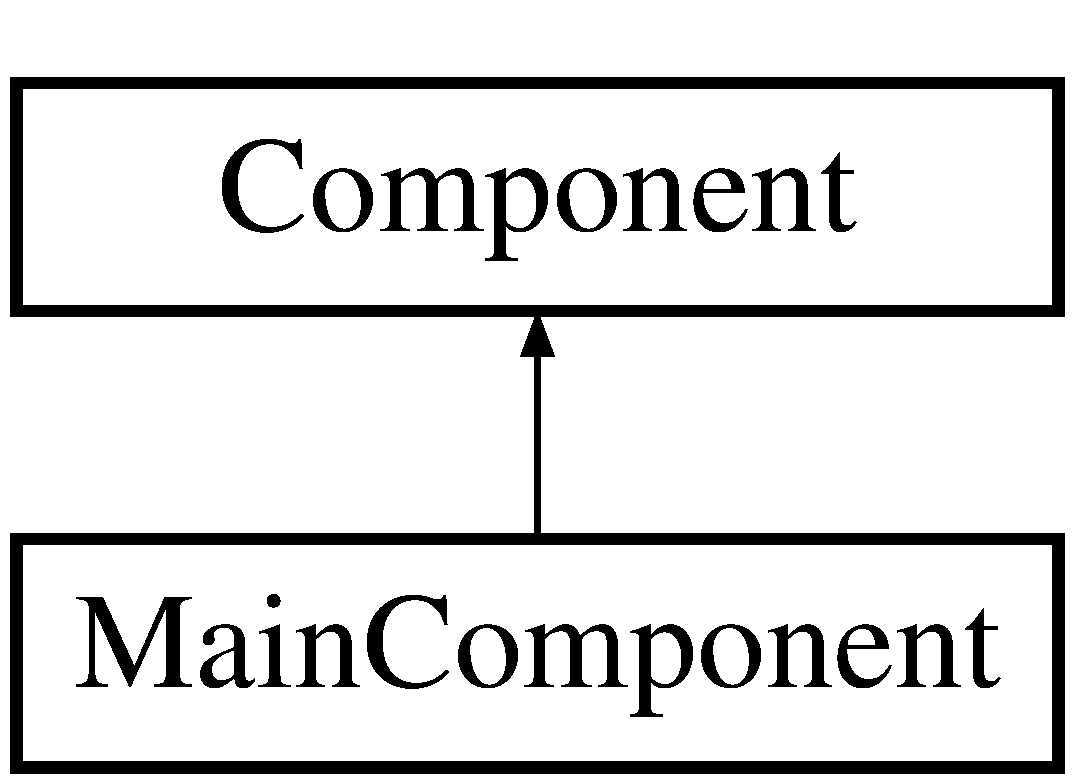
\includegraphics[height=2.000000cm]{class_main_component}
\end{center}
\end{figure}
\subsection*{Public Member Functions}
\begin{DoxyCompactItemize}
\item 
\mbox{\hyperlink{class_main_component_a85254935b98beac9128189c6a577d7be}{Main\+Component}} ()
\item 
\mbox{\hyperlink{class_main_component_aa96a2a286f35edf4000deec5f327d1c3}{$\sim$\+Main\+Component}} ()
\item 
void \mbox{\hyperlink{class_main_component_a413e9316a0332e0522ad69d4f714bfcd}{paint}} (Graphics \&) override
\item 
void \mbox{\hyperlink{class_main_component_a339148bc43089300e10d5883a0a80726}{resized}} () override
\end{DoxyCompactItemize}


\subsection{Detailed Description}


Definition at line 21 of file Main\+Component.\+h.



\subsection{Constructor \& Destructor Documentation}
\mbox{\Hypertarget{class_main_component_a85254935b98beac9128189c6a577d7be}\label{class_main_component_a85254935b98beac9128189c6a577d7be}} 
\index{Main\+Component@{Main\+Component}!Main\+Component@{Main\+Component}}
\index{Main\+Component@{Main\+Component}!Main\+Component@{Main\+Component}}
\subsubsection{\texorpdfstring{Main\+Component()}{MainComponent()}}
{\footnotesize\ttfamily Main\+Component\+::\+Main\+Component (\begin{DoxyParamCaption}{ }\end{DoxyParamCaption})}



Definition at line 12 of file Main\+Component.\+cpp.

\mbox{\Hypertarget{class_main_component_aa96a2a286f35edf4000deec5f327d1c3}\label{class_main_component_aa96a2a286f35edf4000deec5f327d1c3}} 
\index{Main\+Component@{Main\+Component}!````~Main\+Component@{$\sim$\+Main\+Component}}
\index{````~Main\+Component@{$\sim$\+Main\+Component}!Main\+Component@{Main\+Component}}
\subsubsection{\texorpdfstring{$\sim$\+Main\+Component()}{~MainComponent()}}
{\footnotesize\ttfamily Main\+Component\+::$\sim$\+Main\+Component (\begin{DoxyParamCaption}{ }\end{DoxyParamCaption})}



Definition at line 49 of file Main\+Component.\+cpp.



\subsection{Member Function Documentation}
\mbox{\Hypertarget{class_main_component_a413e9316a0332e0522ad69d4f714bfcd}\label{class_main_component_a413e9316a0332e0522ad69d4f714bfcd}} 
\index{Main\+Component@{Main\+Component}!paint@{paint}}
\index{paint@{paint}!Main\+Component@{Main\+Component}}
\subsubsection{\texorpdfstring{paint()}{paint()}}
{\footnotesize\ttfamily void Main\+Component\+::paint (\begin{DoxyParamCaption}\item[{Graphics \&}]{g }\end{DoxyParamCaption})\hspace{0.3cm}{\ttfamily [override]}}



Definition at line 54 of file Main\+Component.\+cpp.

\mbox{\Hypertarget{class_main_component_a339148bc43089300e10d5883a0a80726}\label{class_main_component_a339148bc43089300e10d5883a0a80726}} 
\index{Main\+Component@{Main\+Component}!resized@{resized}}
\index{resized@{resized}!Main\+Component@{Main\+Component}}
\subsubsection{\texorpdfstring{resized()}{resized()}}
{\footnotesize\ttfamily void Main\+Component\+::resized (\begin{DoxyParamCaption}{ }\end{DoxyParamCaption})\hspace{0.3cm}{\ttfamily [override]}}



Definition at line 63 of file Main\+Component.\+cpp.



The documentation for this class was generated from the following files\+:\begin{DoxyCompactItemize}
\item 
Source/\mbox{\hyperlink{_main_component_8h}{Main\+Component.\+h}}\item 
Source/\mbox{\hyperlink{_main_component_8cpp}{Main\+Component.\+cpp}}\end{DoxyCompactItemize}

\hypertarget{class_react_native_j_u_c_e_step1_application_1_1_main_window}{}\section{React\+Native\+J\+U\+C\+E\+Step1\+Application\+:\+:Main\+Window Class Reference}
\label{class_react_native_j_u_c_e_step1_application_1_1_main_window}\index{React\+Native\+J\+U\+C\+E\+Step1\+Application\+::\+Main\+Window@{React\+Native\+J\+U\+C\+E\+Step1\+Application\+::\+Main\+Window}}
Inheritance diagram for React\+Native\+J\+U\+C\+E\+Step1\+Application\+:\+:Main\+Window\+:\begin{figure}[H]
\begin{center}
\leavevmode
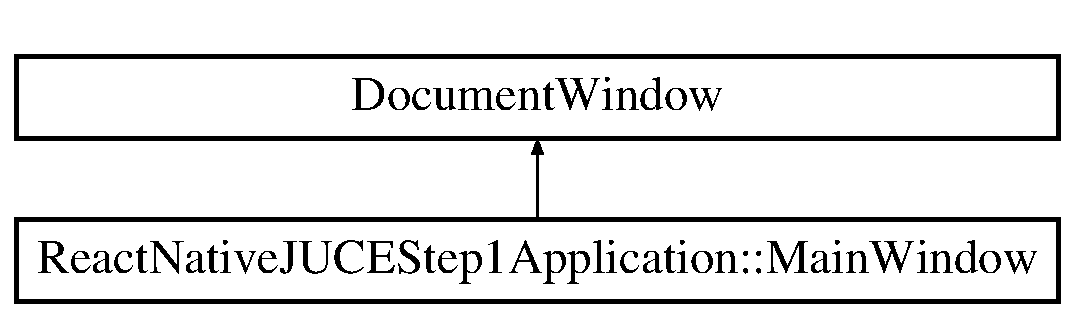
\includegraphics[height=2.000000cm]{class_react_native_j_u_c_e_step1_application_1_1_main_window}
\end{center}
\end{figure}
\subsection*{Public Member Functions}
\begin{DoxyCompactItemize}
\item 
\mbox{\hyperlink{class_react_native_j_u_c_e_step1_application_1_1_main_window_a6d5c670ed3502233b2d5265860a148df}{Main\+Window}} (String name)
\item 
void \mbox{\hyperlink{class_react_native_j_u_c_e_step1_application_1_1_main_window_a46285ddeeb829fd29e5498e504c0e615}{close\+Button\+Pressed}} () override
\end{DoxyCompactItemize}


\subsection{Detailed Description}


Definition at line 60 of file Main.\+cpp.



\subsection{Constructor \& Destructor Documentation}
\mbox{\Hypertarget{class_react_native_j_u_c_e_step1_application_1_1_main_window_a6d5c670ed3502233b2d5265860a148df}\label{class_react_native_j_u_c_e_step1_application_1_1_main_window_a6d5c670ed3502233b2d5265860a148df}} 
\index{React\+Native\+J\+U\+C\+E\+Step1\+Application\+::\+Main\+Window@{React\+Native\+J\+U\+C\+E\+Step1\+Application\+::\+Main\+Window}!Main\+Window@{Main\+Window}}
\index{Main\+Window@{Main\+Window}!React\+Native\+J\+U\+C\+E\+Step1\+Application\+::\+Main\+Window@{React\+Native\+J\+U\+C\+E\+Step1\+Application\+::\+Main\+Window}}
\subsubsection{\texorpdfstring{Main\+Window()}{MainWindow()}}
{\footnotesize\ttfamily React\+Native\+J\+U\+C\+E\+Step1\+Application\+::\+Main\+Window\+::\+Main\+Window (\begin{DoxyParamCaption}\item[{String}]{name }\end{DoxyParamCaption})\hspace{0.3cm}{\ttfamily [inline]}}



Definition at line 63 of file Main.\+cpp.



\subsection{Member Function Documentation}
\mbox{\Hypertarget{class_react_native_j_u_c_e_step1_application_1_1_main_window_a46285ddeeb829fd29e5498e504c0e615}\label{class_react_native_j_u_c_e_step1_application_1_1_main_window_a46285ddeeb829fd29e5498e504c0e615}} 
\index{React\+Native\+J\+U\+C\+E\+Step1\+Application\+::\+Main\+Window@{React\+Native\+J\+U\+C\+E\+Step1\+Application\+::\+Main\+Window}!close\+Button\+Pressed@{close\+Button\+Pressed}}
\index{close\+Button\+Pressed@{close\+Button\+Pressed}!React\+Native\+J\+U\+C\+E\+Step1\+Application\+::\+Main\+Window@{React\+Native\+J\+U\+C\+E\+Step1\+Application\+::\+Main\+Window}}
\subsubsection{\texorpdfstring{close\+Button\+Pressed()}{closeButtonPressed()}}
{\footnotesize\ttfamily void React\+Native\+J\+U\+C\+E\+Step1\+Application\+::\+Main\+Window\+::close\+Button\+Pressed (\begin{DoxyParamCaption}{ }\end{DoxyParamCaption})\hspace{0.3cm}{\ttfamily [inline]}, {\ttfamily [override]}}



Definition at line 81 of file Main.\+cpp.



The documentation for this class was generated from the following file\+:\begin{DoxyCompactItemize}
\item 
Source/\mbox{\hyperlink{_main_8cpp}{Main.\+cpp}}\end{DoxyCompactItemize}

\hypertarget{structcpp__javascriptcore_1_1_null_literal}{}\section{cpp\+\_\+javascriptcore\+:\+:Null\+Literal Struct Reference}
\label{structcpp__javascriptcore_1_1_null_literal}\index{cpp\+\_\+javascriptcore\+::\+Null\+Literal@{cpp\+\_\+javascriptcore\+::\+Null\+Literal}}


{\ttfamily \#include $<$C\+J\+S\+Util.\+h$>$}



\subsection{Detailed Description}


Definition at line 13 of file C\+J\+S\+Util.\+h.



The documentation for this struct was generated from the following file\+:\begin{DoxyCompactItemize}
\item 
Source/\+Cpp-\/\+Java\+Script\+Core/\mbox{\hyperlink{_c_j_s_util_8h}{C\+J\+S\+Util.\+h}}\end{DoxyCompactItemize}

\hypertarget{class_react_native_j_u_c_e_step1_application}{}\section{React\+Native\+J\+U\+C\+E\+Step1\+Application Class Reference}
\label{class_react_native_j_u_c_e_step1_application}\index{React\+Native\+J\+U\+C\+E\+Step1\+Application@{React\+Native\+J\+U\+C\+E\+Step1\+Application}}
Inheritance diagram for React\+Native\+J\+U\+C\+E\+Step1\+Application\+:\begin{figure}[H]
\begin{center}
\leavevmode
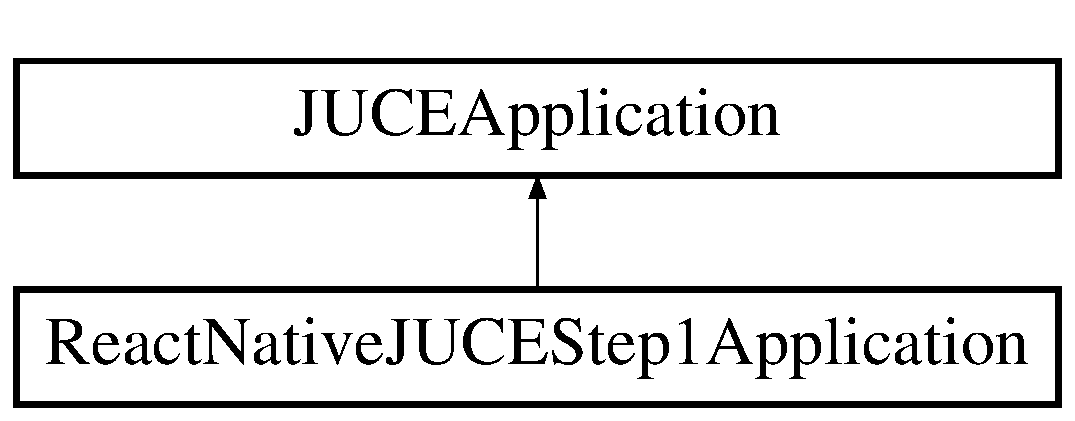
\includegraphics[height=2.000000cm]{class_react_native_j_u_c_e_step1_application}
\end{center}
\end{figure}
\subsection*{Classes}
\begin{DoxyCompactItemize}
\item 
class \mbox{\hyperlink{class_react_native_j_u_c_e_step1_application_1_1_main_window}{Main\+Window}}
\end{DoxyCompactItemize}
\subsection*{Public Member Functions}
\begin{DoxyCompactItemize}
\item 
\mbox{\hyperlink{class_react_native_j_u_c_e_step1_application_a214f8a96e71f6611a185dcd70d0ad87a}{React\+Native\+J\+U\+C\+E\+Step1\+Application}} ()
\item 
const String \mbox{\hyperlink{class_react_native_j_u_c_e_step1_application_adcc1e5f857a72bed3783e31f465ff08c}{get\+Application\+Name}} () override
\item 
const String \mbox{\hyperlink{class_react_native_j_u_c_e_step1_application_a8c374c3a27af7aafab2cc6c294fea893}{get\+Application\+Version}} () override
\item 
bool \mbox{\hyperlink{class_react_native_j_u_c_e_step1_application_a51356d9330ab737202ee4a770d0724d2}{more\+Than\+One\+Instance\+Allowed}} () override
\item 
void \mbox{\hyperlink{class_react_native_j_u_c_e_step1_application_aab55019b53a2ce40f8245d0b18e6d4a5}{initialise}} (const String \&command\+Line) override
\item 
void \mbox{\hyperlink{class_react_native_j_u_c_e_step1_application_ab8d5118377fbb44016543b311e42b07c}{shutdown}} () override
\item 
void \mbox{\hyperlink{class_react_native_j_u_c_e_step1_application_a6e83d2c83b4d58b743f1f168622eb5a0}{system\+Requested\+Quit}} () override
\item 
void \mbox{\hyperlink{class_react_native_j_u_c_e_step1_application_a27d5dfd9ca82a8caafca191dbecdab22}{another\+Instance\+Started}} (const String \&command\+Line) override
\end{DoxyCompactItemize}


\subsection{Detailed Description}


Definition at line 15 of file Main.\+cpp.



\subsection{Constructor \& Destructor Documentation}
\mbox{\Hypertarget{class_react_native_j_u_c_e_step1_application_a214f8a96e71f6611a185dcd70d0ad87a}\label{class_react_native_j_u_c_e_step1_application_a214f8a96e71f6611a185dcd70d0ad87a}} 
\index{React\+Native\+J\+U\+C\+E\+Step1\+Application@{React\+Native\+J\+U\+C\+E\+Step1\+Application}!React\+Native\+J\+U\+C\+E\+Step1\+Application@{React\+Native\+J\+U\+C\+E\+Step1\+Application}}
\index{React\+Native\+J\+U\+C\+E\+Step1\+Application@{React\+Native\+J\+U\+C\+E\+Step1\+Application}!React\+Native\+J\+U\+C\+E\+Step1\+Application@{React\+Native\+J\+U\+C\+E\+Step1\+Application}}
\subsubsection{\texorpdfstring{React\+Native\+J\+U\+C\+E\+Step1\+Application()}{ReactNativeJUCEStep1Application()}}
{\footnotesize\ttfamily React\+Native\+J\+U\+C\+E\+Step1\+Application\+::\+React\+Native\+J\+U\+C\+E\+Step1\+Application (\begin{DoxyParamCaption}{ }\end{DoxyParamCaption})\hspace{0.3cm}{\ttfamily [inline]}}



Definition at line 19 of file Main.\+cpp.



\subsection{Member Function Documentation}
\mbox{\Hypertarget{class_react_native_j_u_c_e_step1_application_a27d5dfd9ca82a8caafca191dbecdab22}\label{class_react_native_j_u_c_e_step1_application_a27d5dfd9ca82a8caafca191dbecdab22}} 
\index{React\+Native\+J\+U\+C\+E\+Step1\+Application@{React\+Native\+J\+U\+C\+E\+Step1\+Application}!another\+Instance\+Started@{another\+Instance\+Started}}
\index{another\+Instance\+Started@{another\+Instance\+Started}!React\+Native\+J\+U\+C\+E\+Step1\+Application@{React\+Native\+J\+U\+C\+E\+Step1\+Application}}
\subsubsection{\texorpdfstring{another\+Instance\+Started()}{anotherInstanceStarted()}}
{\footnotesize\ttfamily void React\+Native\+J\+U\+C\+E\+Step1\+Application\+::another\+Instance\+Started (\begin{DoxyParamCaption}\item[{const String \&}]{command\+Line }\end{DoxyParamCaption})\hspace{0.3cm}{\ttfamily [inline]}, {\ttfamily [override]}}



Definition at line 48 of file Main.\+cpp.

\mbox{\Hypertarget{class_react_native_j_u_c_e_step1_application_adcc1e5f857a72bed3783e31f465ff08c}\label{class_react_native_j_u_c_e_step1_application_adcc1e5f857a72bed3783e31f465ff08c}} 
\index{React\+Native\+J\+U\+C\+E\+Step1\+Application@{React\+Native\+J\+U\+C\+E\+Step1\+Application}!get\+Application\+Name@{get\+Application\+Name}}
\index{get\+Application\+Name@{get\+Application\+Name}!React\+Native\+J\+U\+C\+E\+Step1\+Application@{React\+Native\+J\+U\+C\+E\+Step1\+Application}}
\subsubsection{\texorpdfstring{get\+Application\+Name()}{getApplicationName()}}
{\footnotesize\ttfamily const String React\+Native\+J\+U\+C\+E\+Step1\+Application\+::get\+Application\+Name (\begin{DoxyParamCaption}{ }\end{DoxyParamCaption})\hspace{0.3cm}{\ttfamily [inline]}, {\ttfamily [override]}}



Definition at line 21 of file Main.\+cpp.

\mbox{\Hypertarget{class_react_native_j_u_c_e_step1_application_a8c374c3a27af7aafab2cc6c294fea893}\label{class_react_native_j_u_c_e_step1_application_a8c374c3a27af7aafab2cc6c294fea893}} 
\index{React\+Native\+J\+U\+C\+E\+Step1\+Application@{React\+Native\+J\+U\+C\+E\+Step1\+Application}!get\+Application\+Version@{get\+Application\+Version}}
\index{get\+Application\+Version@{get\+Application\+Version}!React\+Native\+J\+U\+C\+E\+Step1\+Application@{React\+Native\+J\+U\+C\+E\+Step1\+Application}}
\subsubsection{\texorpdfstring{get\+Application\+Version()}{getApplicationVersion()}}
{\footnotesize\ttfamily const String React\+Native\+J\+U\+C\+E\+Step1\+Application\+::get\+Application\+Version (\begin{DoxyParamCaption}{ }\end{DoxyParamCaption})\hspace{0.3cm}{\ttfamily [inline]}, {\ttfamily [override]}}



Definition at line 22 of file Main.\+cpp.

\mbox{\Hypertarget{class_react_native_j_u_c_e_step1_application_aab55019b53a2ce40f8245d0b18e6d4a5}\label{class_react_native_j_u_c_e_step1_application_aab55019b53a2ce40f8245d0b18e6d4a5}} 
\index{React\+Native\+J\+U\+C\+E\+Step1\+Application@{React\+Native\+J\+U\+C\+E\+Step1\+Application}!initialise@{initialise}}
\index{initialise@{initialise}!React\+Native\+J\+U\+C\+E\+Step1\+Application@{React\+Native\+J\+U\+C\+E\+Step1\+Application}}
\subsubsection{\texorpdfstring{initialise()}{initialise()}}
{\footnotesize\ttfamily void React\+Native\+J\+U\+C\+E\+Step1\+Application\+::initialise (\begin{DoxyParamCaption}\item[{const String \&}]{command\+Line }\end{DoxyParamCaption})\hspace{0.3cm}{\ttfamily [inline]}, {\ttfamily [override]}}



Definition at line 26 of file Main.\+cpp.

\mbox{\Hypertarget{class_react_native_j_u_c_e_step1_application_a51356d9330ab737202ee4a770d0724d2}\label{class_react_native_j_u_c_e_step1_application_a51356d9330ab737202ee4a770d0724d2}} 
\index{React\+Native\+J\+U\+C\+E\+Step1\+Application@{React\+Native\+J\+U\+C\+E\+Step1\+Application}!more\+Than\+One\+Instance\+Allowed@{more\+Than\+One\+Instance\+Allowed}}
\index{more\+Than\+One\+Instance\+Allowed@{more\+Than\+One\+Instance\+Allowed}!React\+Native\+J\+U\+C\+E\+Step1\+Application@{React\+Native\+J\+U\+C\+E\+Step1\+Application}}
\subsubsection{\texorpdfstring{more\+Than\+One\+Instance\+Allowed()}{moreThanOneInstanceAllowed()}}
{\footnotesize\ttfamily bool React\+Native\+J\+U\+C\+E\+Step1\+Application\+::more\+Than\+One\+Instance\+Allowed (\begin{DoxyParamCaption}{ }\end{DoxyParamCaption})\hspace{0.3cm}{\ttfamily [inline]}, {\ttfamily [override]}}



Definition at line 23 of file Main.\+cpp.

\mbox{\Hypertarget{class_react_native_j_u_c_e_step1_application_ab8d5118377fbb44016543b311e42b07c}\label{class_react_native_j_u_c_e_step1_application_ab8d5118377fbb44016543b311e42b07c}} 
\index{React\+Native\+J\+U\+C\+E\+Step1\+Application@{React\+Native\+J\+U\+C\+E\+Step1\+Application}!shutdown@{shutdown}}
\index{shutdown@{shutdown}!React\+Native\+J\+U\+C\+E\+Step1\+Application@{React\+Native\+J\+U\+C\+E\+Step1\+Application}}
\subsubsection{\texorpdfstring{shutdown()}{shutdown()}}
{\footnotesize\ttfamily void React\+Native\+J\+U\+C\+E\+Step1\+Application\+::shutdown (\begin{DoxyParamCaption}{ }\end{DoxyParamCaption})\hspace{0.3cm}{\ttfamily [inline]}, {\ttfamily [override]}}



Definition at line 33 of file Main.\+cpp.

\mbox{\Hypertarget{class_react_native_j_u_c_e_step1_application_a6e83d2c83b4d58b743f1f168622eb5a0}\label{class_react_native_j_u_c_e_step1_application_a6e83d2c83b4d58b743f1f168622eb5a0}} 
\index{React\+Native\+J\+U\+C\+E\+Step1\+Application@{React\+Native\+J\+U\+C\+E\+Step1\+Application}!system\+Requested\+Quit@{system\+Requested\+Quit}}
\index{system\+Requested\+Quit@{system\+Requested\+Quit}!React\+Native\+J\+U\+C\+E\+Step1\+Application@{React\+Native\+J\+U\+C\+E\+Step1\+Application}}
\subsubsection{\texorpdfstring{system\+Requested\+Quit()}{systemRequestedQuit()}}
{\footnotesize\ttfamily void React\+Native\+J\+U\+C\+E\+Step1\+Application\+::system\+Requested\+Quit (\begin{DoxyParamCaption}{ }\end{DoxyParamCaption})\hspace{0.3cm}{\ttfamily [inline]}, {\ttfamily [override]}}



Definition at line 41 of file Main.\+cpp.



The documentation for this class was generated from the following file\+:\begin{DoxyCompactItemize}
\item 
Source/\mbox{\hyperlink{_main_8cpp}{Main.\+cpp}}\end{DoxyCompactItemize}

\hypertarget{structcpp__javascriptcore_1_1_undefined_literal}{}\section{cpp\+\_\+javascriptcore\+:\+:Undefined\+Literal Struct Reference}
\label{structcpp__javascriptcore_1_1_undefined_literal}\index{cpp\+\_\+javascriptcore\+::\+Undefined\+Literal@{cpp\+\_\+javascriptcore\+::\+Undefined\+Literal}}


{\ttfamily \#include $<$C\+J\+S\+Util.\+h$>$}



\subsection{Detailed Description}


Definition at line 9 of file C\+J\+S\+Util.\+h.



The documentation for this struct was generated from the following file\+:\begin{DoxyCompactItemize}
\item 
Source/\+Cpp-\/\+Java\+Script\+Core/\mbox{\hyperlink{_c_j_s_util_8h}{C\+J\+S\+Util.\+h}}\end{DoxyCompactItemize}

\chapter{File Documentation}
\hypertarget{_c_j_s_class_8h}{}\section{Source/\+Cpp-\/\+Java\+Script\+Core/\+C\+J\+S\+Class.h File Reference}
\label{_c_j_s_class_8h}\index{Source/\+Cpp-\/\+Java\+Script\+Core/\+C\+J\+S\+Class.\+h@{Source/\+Cpp-\/\+Java\+Script\+Core/\+C\+J\+S\+Class.\+h}}
{\ttfamily \#include $<$Java\+Script\+Core/\+Java\+Script\+Core.\+h$>$}\newline
{\ttfamily \#include $<$functional$>$}\newline
{\ttfamily \#include $<$unordered\+\_\+map$>$}\newline
\subsection*{Classes}
\begin{DoxyCompactItemize}
\item 
class \mbox{\hyperlink{classcpp__javascriptcore_1_1_c_j_s_class}{cpp\+\_\+javascriptcore\+::\+C\+J\+S\+Class}}
\end{DoxyCompactItemize}
\subsection*{Namespaces}
\begin{DoxyCompactItemize}
\item 
 \mbox{\hyperlink{namespacecpp__javascriptcore}{cpp\+\_\+javascriptcore}}
\end{DoxyCompactItemize}

\hypertarget{_c_j_s_constructor_8cpp}{}\section{Source/\+Cpp-\/\+Java\+Script\+Core/\+C\+J\+S\+Constructor.cpp File Reference}
\label{_c_j_s_constructor_8cpp}\index{Source/\+Cpp-\/\+Java\+Script\+Core/\+C\+J\+S\+Constructor.\+cpp@{Source/\+Cpp-\/\+Java\+Script\+Core/\+C\+J\+S\+Constructor.\+cpp}}
{\ttfamily \#include \char`\"{}C\+J\+S\+Constructor.\+h\char`\"{}}\newline
\subsection*{Namespaces}
\begin{DoxyCompactItemize}
\item 
 \mbox{\hyperlink{namespacecpp__javascriptcore}{cpp\+\_\+javascriptcore}}
\end{DoxyCompactItemize}

\hypertarget{_c_j_s_constructor_8h}{}\section{Source/\+Cpp-\/\+Java\+Script\+Core/\+C\+J\+S\+Constructor.h File Reference}
\label{_c_j_s_constructor_8h}\index{Source/\+Cpp-\/\+Java\+Script\+Core/\+C\+J\+S\+Constructor.\+h@{Source/\+Cpp-\/\+Java\+Script\+Core/\+C\+J\+S\+Constructor.\+h}}
{\ttfamily \#include $<$Java\+Script\+Core/\+Java\+Script\+Core.\+h$>$}\newline
{\ttfamily \#include $<$functional$>$}\newline
{\ttfamily \#include $<$unordered\+\_\+map$>$}\newline
\subsection*{Classes}
\begin{DoxyCompactItemize}
\item 
class \mbox{\hyperlink{classcpp__javascriptcore_1_1_c_j_s_constructor}{cpp\+\_\+javascriptcore\+::\+C\+J\+S\+Constructor}}
\end{DoxyCompactItemize}
\subsection*{Namespaces}
\begin{DoxyCompactItemize}
\item 
 \mbox{\hyperlink{namespacecpp__javascriptcore}{cpp\+\_\+javascriptcore}}
\end{DoxyCompactItemize}

\hypertarget{_c_j_s_export_class_8h}{}\section{Source/\+Cpp-\/\+Java\+Script\+Core/\+C\+J\+S\+Export\+Class.h File Reference}
\label{_c_j_s_export_class_8h}\index{Source/\+Cpp-\/\+Java\+Script\+Core/\+C\+J\+S\+Export\+Class.\+h@{Source/\+Cpp-\/\+Java\+Script\+Core/\+C\+J\+S\+Export\+Class.\+h}}
{\ttfamily \#include $<$string$>$}\newline
\subsection*{Classes}
\begin{DoxyCompactItemize}
\item 
class \mbox{\hyperlink{class_c_j_s_export_builder}{C\+J\+S\+Export\+Builder}}
\end{DoxyCompactItemize}
\subsection*{Functions}
\begin{DoxyCompactItemize}
\item 
{\footnotesize template$<$typename T $>$ }\\\mbox{\hyperlink{class_c_j_s_export_builder}{C\+J\+S\+Export\+Builder}} \mbox{\hyperlink{_c_j_s_export_class_8h_a5a55051ee972cb68683d922de801f1d7}{class\+\_\+}} (std\+::string class\+Name)
\end{DoxyCompactItemize}


\subsection{Function Documentation}
\mbox{\Hypertarget{_c_j_s_export_class_8h_a5a55051ee972cb68683d922de801f1d7}\label{_c_j_s_export_class_8h_a5a55051ee972cb68683d922de801f1d7}} 
\index{C\+J\+S\+Export\+Class.\+h@{C\+J\+S\+Export\+Class.\+h}!class\+\_\+@{class\+\_\+}}
\index{class\+\_\+@{class\+\_\+}!C\+J\+S\+Export\+Class.\+h@{C\+J\+S\+Export\+Class.\+h}}
\subsubsection{\texorpdfstring{class\+\_\+()}{class\_()}}
{\footnotesize\ttfamily template$<$typename T $>$ \\
\mbox{\hyperlink{class_c_j_s_export_builder}{C\+J\+S\+Export\+Builder}} class\+\_\+ (\begin{DoxyParamCaption}\item[{std\+::string}]{class\+Name }\end{DoxyParamCaption})}



Definition at line 9 of file C\+J\+S\+Export\+Class.\+h.


\hypertarget{_c_j_s_function_8cpp}{}\section{Source/\+Cpp-\/\+Java\+Script\+Core/\+C\+J\+S\+Function.cpp File Reference}
\label{_c_j_s_function_8cpp}\index{Source/\+Cpp-\/\+Java\+Script\+Core/\+C\+J\+S\+Function.\+cpp@{Source/\+Cpp-\/\+Java\+Script\+Core/\+C\+J\+S\+Function.\+cpp}}
{\ttfamily \#include \char`\"{}C\+J\+S\+Function.\+h\char`\"{}}\newline
\subsection*{Namespaces}
\begin{DoxyCompactItemize}
\item 
 \mbox{\hyperlink{namespacecpp__javascriptcore}{cpp\+\_\+javascriptcore}}
\end{DoxyCompactItemize}

\hypertarget{_c_j_s_function_8h}{}\section{Source/\+Cpp-\/\+Java\+Script\+Core/\+C\+J\+S\+Function.h File Reference}
\label{_c_j_s_function_8h}\index{Source/\+Cpp-\/\+Java\+Script\+Core/\+C\+J\+S\+Function.\+h@{Source/\+Cpp-\/\+Java\+Script\+Core/\+C\+J\+S\+Function.\+h}}
{\ttfamily \#include $<$Java\+Script\+Core/\+Java\+Script\+Core.\+h$>$}\newline
{\ttfamily \#include $<$functional$>$}\newline
{\ttfamily \#include $<$optional$>$}\newline
{\ttfamily \#include $<$string$>$}\newline
{\ttfamily \#include $<$unordered\+\_\+map$>$}\newline
{\ttfamily \#include $<$iostream$>$}\newline
{\ttfamily \#include \char`\"{}C\+J\+S\+Util.\+h\char`\"{}}\newline
\subsection*{Classes}
\begin{DoxyCompactItemize}
\item 
class \mbox{\hyperlink{classcpp__javascriptcore_1_1_c_j_s_function}{cpp\+\_\+javascriptcore\+::\+C\+J\+S\+Function}}
\end{DoxyCompactItemize}
\subsection*{Namespaces}
\begin{DoxyCompactItemize}
\item 
 \mbox{\hyperlink{namespacecpp__javascriptcore}{cpp\+\_\+javascriptcore}}
\end{DoxyCompactItemize}
\subsection*{Typedefs}
\begin{DoxyCompactItemize}
\item 
using \mbox{\hyperlink{namespacecpp__javascriptcore_ade392e059225cd35b14b1b7efb9d5a5b}{cpp\+\_\+javascriptcore\+::\+Cb\+J\+S\+Args\+Returning\+J\+S\+Value\+With\+Context}} = std\+::function$<$ J\+S\+Value\+Ref(J\+S\+Context\+Ref, J\+S\+Object\+Ref, size\+\_\+t, const J\+S\+Value\+Ref\mbox{[}$\,$\mbox{]})$>$
\end{DoxyCompactItemize}

\hypertarget{_c_j_s_object_8cpp}{}\section{Source/\+Cpp-\/\+Java\+Script\+Core/\+C\+J\+S\+Object.cpp File Reference}
\label{_c_j_s_object_8cpp}\index{Source/\+Cpp-\/\+Java\+Script\+Core/\+C\+J\+S\+Object.\+cpp@{Source/\+Cpp-\/\+Java\+Script\+Core/\+C\+J\+S\+Object.\+cpp}}
{\ttfamily \#include \char`\"{}C\+J\+S\+Object.\+h\char`\"{}}\newline
\subsection*{Namespaces}
\begin{DoxyCompactItemize}
\item 
 \mbox{\hyperlink{namespacecpp__javascriptcore}{cpp\+\_\+javascriptcore}}
\end{DoxyCompactItemize}

\hypertarget{_c_j_s_object_8h}{}\section{Source/\+Cpp-\/\+Java\+Script\+Core/\+C\+J\+S\+Object.h File Reference}
\label{_c_j_s_object_8h}\index{Source/\+Cpp-\/\+Java\+Script\+Core/\+C\+J\+S\+Object.\+h@{Source/\+Cpp-\/\+Java\+Script\+Core/\+C\+J\+S\+Object.\+h}}
{\ttfamily \#include $<$Java\+Script\+Core/\+Java\+Script\+Core.\+h$>$}\newline
{\ttfamily \#include $<$neither/\+Either.\+hpp$>$}\newline
{\ttfamily \#include \char`\"{}C\+J\+S\+Class.\+h\char`\"{}}\newline
{\ttfamily \#include \char`\"{}C\+J\+S\+Util.\+h\char`\"{}}\newline
{\ttfamily \#include \char`\"{}C\+J\+S\+Value.\+h\char`\"{}}\newline
{\ttfamily \#include \char`\"{}Magic\+Conversion.\+h\char`\"{}}\newline
\subsection*{Classes}
\begin{DoxyCompactItemize}
\item 
class \mbox{\hyperlink{classcpp__javascriptcore_1_1_c_j_s_object}{cpp\+\_\+javascriptcore\+::\+C\+J\+S\+Object}}
\end{DoxyCompactItemize}
\subsection*{Namespaces}
\begin{DoxyCompactItemize}
\item 
 \mbox{\hyperlink{namespacecpp__javascriptcore}{cpp\+\_\+javascriptcore}}
\end{DoxyCompactItemize}

\hypertarget{_c_j_s_util_8cpp}{}\section{Source/\+Cpp-\/\+Java\+Script\+Core/\+C\+J\+S\+Util.cpp File Reference}
\label{_c_j_s_util_8cpp}\index{Source/\+Cpp-\/\+Java\+Script\+Core/\+C\+J\+S\+Util.\+cpp@{Source/\+Cpp-\/\+Java\+Script\+Core/\+C\+J\+S\+Util.\+cpp}}
{\ttfamily \#include \char`\"{}C\+J\+S\+Util.\+h\char`\"{}}\newline
\subsection*{Namespaces}
\begin{DoxyCompactItemize}
\item 
 \mbox{\hyperlink{namespacecpp__javascriptcore}{cpp\+\_\+javascriptcore}}
\end{DoxyCompactItemize}
\subsection*{Functions}
\begin{DoxyCompactItemize}
\item 
J\+S\+String\+Ref \mbox{\hyperlink{namespacecpp__javascriptcore_a64c0a5a8f178db673f0eb7704ee78816}{cpp\+\_\+javascriptcore\+::get\+J\+S\+String\+Ref\+From\+String}} (const std\+::string \&str)
\end{DoxyCompactItemize}

\hypertarget{_c_j_s_util_8h}{}\section{Source/\+Cpp-\/\+Java\+Script\+Core/\+C\+J\+S\+Util.h File Reference}
\label{_c_j_s_util_8h}\index{Source/\+Cpp-\/\+Java\+Script\+Core/\+C\+J\+S\+Util.\+h@{Source/\+Cpp-\/\+Java\+Script\+Core/\+C\+J\+S\+Util.\+h}}
{\ttfamily \#include $<$Java\+Script\+Core/\+Java\+Script\+Core.\+h$>$}\newline
{\ttfamily \#include $<$string$>$}\newline
\subsection*{Classes}
\begin{DoxyCompactItemize}
\item 
struct \mbox{\hyperlink{structcpp__javascriptcore_1_1_undefined_literal}{cpp\+\_\+javascriptcore\+::\+Undefined\+Literal}}
\item 
struct \mbox{\hyperlink{structcpp__javascriptcore_1_1_null_literal}{cpp\+\_\+javascriptcore\+::\+Null\+Literal}}
\end{DoxyCompactItemize}
\subsection*{Namespaces}
\begin{DoxyCompactItemize}
\item 
 \mbox{\hyperlink{namespacecpp__javascriptcore}{cpp\+\_\+javascriptcore}}
\end{DoxyCompactItemize}
\subsection*{Functions}
\begin{DoxyCompactItemize}
\item 
J\+S\+String\+Ref \mbox{\hyperlink{namespacecpp__javascriptcore_a64c0a5a8f178db673f0eb7704ee78816}{cpp\+\_\+javascriptcore\+::get\+J\+S\+String\+Ref\+From\+String}} (const std\+::string \&str)
\end{DoxyCompactItemize}

\hypertarget{_c_j_s_value_8cpp}{}\section{Source/\+Cpp-\/\+Java\+Script\+Core/\+C\+J\+S\+Value.cpp File Reference}
\label{_c_j_s_value_8cpp}\index{Source/\+Cpp-\/\+Java\+Script\+Core/\+C\+J\+S\+Value.\+cpp@{Source/\+Cpp-\/\+Java\+Script\+Core/\+C\+J\+S\+Value.\+cpp}}
{\ttfamily \#include \char`\"{}C\+J\+S\+Value.\+h\char`\"{}}\newline
{\ttfamily \#include \char`\"{}C\+J\+S\+Object.\+h\char`\"{}}\newline
\subsection*{Namespaces}
\begin{DoxyCompactItemize}
\item 
 \mbox{\hyperlink{namespacecpp__javascriptcore}{cpp\+\_\+javascriptcore}}
\end{DoxyCompactItemize}

\hypertarget{_c_j_s_value_8h}{}\section{Source/\+Cpp-\/\+Java\+Script\+Core/\+C\+J\+S\+Value.h File Reference}
\label{_c_j_s_value_8h}\index{Source/\+Cpp-\/\+Java\+Script\+Core/\+C\+J\+S\+Value.\+h@{Source/\+Cpp-\/\+Java\+Script\+Core/\+C\+J\+S\+Value.\+h}}
{\ttfamily \#include $<$Java\+Script\+Core/\+Java\+Script\+Core.\+h$>$}\newline
{\ttfamily \#include $<$neither/\+Either.\+hpp$>$}\newline
{\ttfamily \#include $<$string$>$}\newline
\subsection*{Classes}
\begin{DoxyCompactItemize}
\item 
class \mbox{\hyperlink{classcpp__javascriptcore_1_1_c_j_s_value}{cpp\+\_\+javascriptcore\+::\+C\+J\+S\+Value}}
\end{DoxyCompactItemize}
\subsection*{Namespaces}
\begin{DoxyCompactItemize}
\item 
 \mbox{\hyperlink{namespacecpp__javascriptcore}{cpp\+\_\+javascriptcore}}
\end{DoxyCompactItemize}

\hypertarget{_cpp-_java_script_core_8cpp}{}\section{Source/\+Cpp-\/\+Java\+Script\+Core/\+Cpp-\/\+Java\+Script\+Core.cpp File Reference}
\label{_cpp-_java_script_core_8cpp}\index{Source/\+Cpp-\/\+Java\+Script\+Core/\+Cpp-\/\+Java\+Script\+Core.\+cpp@{Source/\+Cpp-\/\+Java\+Script\+Core/\+Cpp-\/\+Java\+Script\+Core.\+cpp}}
{\ttfamily \#include \char`\"{}Cpp-\/\+Java\+Script\+Core.\+h\char`\"{}}\newline
\subsection*{Namespaces}
\begin{DoxyCompactItemize}
\item 
 \mbox{\hyperlink{namespacecpp__javascriptcore}{cpp\+\_\+javascriptcore}}
\end{DoxyCompactItemize}

\hypertarget{_cpp-_java_script_core_8h}{}\section{Source/\+Cpp-\/\+Java\+Script\+Core/\+Cpp-\/\+Java\+Script\+Core.h File Reference}
\label{_cpp-_java_script_core_8h}\index{Source/\+Cpp-\/\+Java\+Script\+Core/\+Cpp-\/\+Java\+Script\+Core.\+h@{Source/\+Cpp-\/\+Java\+Script\+Core/\+Cpp-\/\+Java\+Script\+Core.\+h}}
{\ttfamily \#include $<$Java\+Script\+Core/\+Java\+Script\+Core.\+h$>$}\newline
{\ttfamily \#include $<$functional$>$}\newline
{\ttfamily \#include $<$iostream$>$}\newline
{\ttfamily \#include $<$neither/either.\+hpp$>$}\newline
{\ttfamily \#include $<$optional$>$}\newline
{\ttfamily \#include $<$string$>$}\newline
{\ttfamily \#include \char`\"{}C\+J\+S\+Class.\+h\char`\"{}}\newline
{\ttfamily \#include \char`\"{}C\+J\+S\+Constructor.\+h\char`\"{}}\newline
{\ttfamily \#include \char`\"{}C\+J\+S\+Function.\+h\char`\"{}}\newline
{\ttfamily \#include \char`\"{}C\+J\+S\+Object.\+h\char`\"{}}\newline
{\ttfamily \#include \char`\"{}C\+J\+S\+Value.\+h\char`\"{}}\newline
{\ttfamily \#include \char`\"{}Magic\+Conversion.\+h\char`\"{}}\newline
\subsection*{Classes}
\begin{DoxyCompactItemize}
\item 
class \mbox{\hyperlink{classcpp__javascriptcore_1_1_c_j_s_context}{cpp\+\_\+javascriptcore\+::\+C\+J\+S\+Context}}
\end{DoxyCompactItemize}
\subsection*{Namespaces}
\begin{DoxyCompactItemize}
\item 
 \mbox{\hyperlink{namespacecpp__javascriptcore}{cpp\+\_\+javascriptcore}}
\end{DoxyCompactItemize}

\hypertarget{_magic_conversion_8cpp}{}\section{Source/\+Cpp-\/\+Java\+Script\+Core/\+Magic\+Conversion.cpp File Reference}
\label{_magic_conversion_8cpp}\index{Source/\+Cpp-\/\+Java\+Script\+Core/\+Magic\+Conversion.\+cpp@{Source/\+Cpp-\/\+Java\+Script\+Core/\+Magic\+Conversion.\+cpp}}
{\ttfamily \#include \char`\"{}Magic\+Conversion.\+h\char`\"{}}\newline
\subsection*{Namespaces}
\begin{DoxyCompactItemize}
\item 
 \mbox{\hyperlink{namespacecpp__javascriptcore}{cpp\+\_\+javascriptcore}}
\end{DoxyCompactItemize}
\subsection*{Functions}
\begin{DoxyCompactItemize}
\item 
std\+::vector$<$ J\+S\+Value\+Ref $>$ \mbox{\hyperlink{namespacecpp__javascriptcore_a5d52cd145305a6c024858e80973867e5}{cpp\+\_\+javascriptcore\+::convert\+Values}} (J\+S\+Context\+Ref context)
\end{DoxyCompactItemize}

\hypertarget{_magic_conversion_8h}{}\section{Source/\+Cpp-\/\+Java\+Script\+Core/\+Magic\+Conversion.h File Reference}
\label{_magic_conversion_8h}\index{Source/\+Cpp-\/\+Java\+Script\+Core/\+Magic\+Conversion.\+h@{Source/\+Cpp-\/\+Java\+Script\+Core/\+Magic\+Conversion.\+h}}
{\ttfamily \#include \char`\"{}C\+J\+S\+Function.\+h\char`\"{}}\newline
{\ttfamily \#include \char`\"{}C\+J\+S\+Value.\+h\char`\"{}}\newline
{\ttfamily \#include $<$Java\+Script\+Core/\+Java\+Script\+Core.\+h$>$}\newline
{\ttfamily \#include $<$boost/callable\+\_\+traits.\+hpp$>$}\newline
{\ttfamily \#include $<$tuple$>$}\newline
{\ttfamily \#include $<$vector$>$}\newline
\subsection*{Namespaces}
\begin{DoxyCompactItemize}
\item 
 \mbox{\hyperlink{namespacecpp__javascriptcore}{cpp\+\_\+javascriptcore}}
\end{DoxyCompactItemize}
\subsection*{Functions}
\begin{DoxyCompactItemize}
\item 
{\footnotesize template$<$typename Arg $>$ }\\C\+J\+S\+Value \mbox{\hyperlink{namespacecpp__javascriptcore_a2ae1cd64b14aa12f56f503463a3dede6}{cpp\+\_\+javascriptcore\+::convert\+Value}} (J\+S\+Context\+Ref context, Arg value)
\item 
std\+::vector$<$ J\+S\+Value\+Ref $>$ \mbox{\hyperlink{namespacecpp__javascriptcore_a5d52cd145305a6c024858e80973867e5}{cpp\+\_\+javascriptcore\+::convert\+Values}} (J\+S\+Context\+Ref context)
\item 
{\footnotesize template$<$typename Arg , typename... Args$>$ }\\std\+::vector$<$ J\+S\+Value\+Ref $>$ \mbox{\hyperlink{namespacecpp__javascriptcore_ad53bb2850a23b75e56b6d953fc90b552}{cpp\+\_\+javascriptcore\+::convert\+Values}} (J\+S\+Context\+Ref context, Arg value, Args... tail)
\item 
{\footnotesize template$<$typename Ret $>$ }\\Ret \mbox{\hyperlink{namespacecpp__javascriptcore_a63b8017b1766288a57631889bd4d205c}{cpp\+\_\+javascriptcore\+::from\+JS}} (J\+S\+Context\+Ref context, J\+S\+Value\+Ref value)
\item 
{\footnotesize template$<$typename F , typename Arg\+Types , std\+::size\+\_\+t N, std\+::size\+\_\+t... Idx$>$ }\\decltype(auto) \mbox{\hyperlink{namespacecpp__javascriptcore_a2c32796cd818b3a75a7dc6f033b4a596}{cpp\+\_\+javascriptcore\+::apply\+Impl}} (F fn, Arg\+Types \&args, std\+::index\+\_\+sequence$<$ Idx... $>$)
\item 
{\footnotesize template$<$typename F , typename Arg\+Types , std\+::size\+\_\+t N$>$ }\\decltype(auto) \mbox{\hyperlink{namespacecpp__javascriptcore_ae99580d5a07367766396914230c5cb4a}{cpp\+\_\+javascriptcore\+::apply}} (F fn, Arg\+Types \&args)
\item 
{\footnotesize template$<$typename Fn $>$ }\\C\+J\+S\+Function\+::\+Callback \mbox{\hyperlink{namespacecpp__javascriptcore_ac75c77a83b4f02ba3e0529799f49a313}{cpp\+\_\+javascriptcore\+::make\+Callback}} (Fn \&\&callback)
\end{DoxyCompactItemize}

\hypertarget{_j_s_c-_j_u_c_e_8cpp}{}\section{Source/\+J\+S\+C-\/\+J\+U\+C\+E/\+J\+S\+C-\/\+J\+U\+CE.cpp File Reference}
\label{_j_s_c-_j_u_c_e_8cpp}\index{Source/\+J\+S\+C-\/\+J\+U\+C\+E/\+J\+S\+C-\/\+J\+U\+C\+E.\+cpp@{Source/\+J\+S\+C-\/\+J\+U\+C\+E/\+J\+S\+C-\/\+J\+U\+C\+E.\+cpp}}
{\ttfamily \#include \char`\"{}J\+S\+C-\/\+J\+U\+C\+E.\+h\char`\"{}}\newline
\subsection*{Functions}
\begin{DoxyCompactItemize}
\item 
J\+S\+Object\+Ref \mbox{\hyperlink{_j_s_c-_j_u_c_e_8cpp_a4979f6178ff7382e34f456a6e48b3998}{make\+Component\+Class}} (C\+J\+S\+Context \&context)
\end{DoxyCompactItemize}


\subsection{Function Documentation}
\mbox{\Hypertarget{_j_s_c-_j_u_c_e_8cpp_a4979f6178ff7382e34f456a6e48b3998}\label{_j_s_c-_j_u_c_e_8cpp_a4979f6178ff7382e34f456a6e48b3998}} 
\index{J\+S\+C-\/\+J\+U\+C\+E.\+cpp@{J\+S\+C-\/\+J\+U\+C\+E.\+cpp}!make\+Component\+Class@{make\+Component\+Class}}
\index{make\+Component\+Class@{make\+Component\+Class}!J\+S\+C-\/\+J\+U\+C\+E.\+cpp@{J\+S\+C-\/\+J\+U\+C\+E.\+cpp}}
\subsubsection{\texorpdfstring{make\+Component\+Class()}{makeComponentClass()}}
{\footnotesize\ttfamily J\+S\+Object\+Ref make\+Component\+Class (\begin{DoxyParamCaption}\item[{C\+J\+S\+Context \&}]{context }\end{DoxyParamCaption})}



Definition at line 3 of file J\+S\+C-\/\+J\+U\+C\+E.\+cpp.


\hypertarget{_j_s_c-_j_u_c_e_8h}{}\section{Source/\+J\+S\+C-\/\+J\+U\+C\+E/\+J\+S\+C-\/\+J\+U\+CE.h File Reference}
\label{_j_s_c-_j_u_c_e_8h}\index{Source/\+J\+S\+C-\/\+J\+U\+C\+E/\+J\+S\+C-\/\+J\+U\+C\+E.\+h@{Source/\+J\+S\+C-\/\+J\+U\+C\+E/\+J\+S\+C-\/\+J\+U\+C\+E.\+h}}
{\ttfamily \#include \char`\"{}../\+Cpp-\/\+Java\+Script\+Core/\+Cpp-\/\+Java\+Script\+Core.\+h\char`\"{}}\newline
\subsection*{Functions}
\begin{DoxyCompactItemize}
\item 
J\+S\+Class\+Ref \mbox{\hyperlink{_j_s_c-_j_u_c_e_8h_ab10068264b712931698990ee9a47ce3f}{make\+Component\+Class}} (C\+J\+S\+Context \&context)
\end{DoxyCompactItemize}


\subsection{Function Documentation}
\mbox{\Hypertarget{_j_s_c-_j_u_c_e_8h_ab10068264b712931698990ee9a47ce3f}\label{_j_s_c-_j_u_c_e_8h_ab10068264b712931698990ee9a47ce3f}} 
\index{J\+S\+C-\/\+J\+U\+C\+E.\+h@{J\+S\+C-\/\+J\+U\+C\+E.\+h}!make\+Component\+Class@{make\+Component\+Class}}
\index{make\+Component\+Class@{make\+Component\+Class}!J\+S\+C-\/\+J\+U\+C\+E.\+h@{J\+S\+C-\/\+J\+U\+C\+E.\+h}}
\subsubsection{\texorpdfstring{make\+Component\+Class()}{makeComponentClass()}}
{\footnotesize\ttfamily J\+S\+Class\+Ref make\+Component\+Class (\begin{DoxyParamCaption}\item[{C\+J\+S\+Context \&}]{context }\end{DoxyParamCaption})}



Definition at line 3 of file J\+S\+C-\/\+J\+U\+C\+E.\+cpp.


\hypertarget{_main_8cpp}{}\section{Source/\+Main.cpp File Reference}
\label{_main_8cpp}\index{Source/\+Main.\+cpp@{Source/\+Main.\+cpp}}
{\ttfamily \#include \char`\"{}../\+Juce\+Library\+Code/\+Juce\+Header.\+h\char`\"{}}\newline
{\ttfamily \#include \char`\"{}Main\+Component.\+h\char`\"{}}\newline
\subsection*{Classes}
\begin{DoxyCompactItemize}
\item 
class \mbox{\hyperlink{class_react_native_j_u_c_e_step1_application}{React\+Native\+J\+U\+C\+E\+Step1\+Application}}
\item 
class \mbox{\hyperlink{class_react_native_j_u_c_e_step1_application_1_1_main_window}{React\+Native\+J\+U\+C\+E\+Step1\+Application\+::\+Main\+Window}}
\end{DoxyCompactItemize}

\hypertarget{_main_component_8cpp}{}\section{Source/\+Main\+Component.cpp File Reference}
\label{_main_component_8cpp}\index{Source/\+Main\+Component.\+cpp@{Source/\+Main\+Component.\+cpp}}
{\ttfamily \#include \char`\"{}Main\+Component.\+h\char`\"{}}\newline

\hypertarget{_main_component_8h}{}\section{Source/\+Main\+Component.h File Reference}
\label{_main_component_8h}\index{Source/\+Main\+Component.\+h@{Source/\+Main\+Component.\+h}}
{\ttfamily \#include \char`\"{}../\+Juce\+Library\+Code/\+Juce\+Header.\+h\char`\"{}}\newline
{\ttfamily \#include \char`\"{}Cpp-\/\+Java\+Script\+Core/\+Cpp-\/\+Java\+Script\+Core.\+h\char`\"{}}\newline
\subsection*{Classes}
\begin{DoxyCompactItemize}
\item 
class \mbox{\hyperlink{class_main_component}{Main\+Component}}
\end{DoxyCompactItemize}

%--- End generated contents ---

% Index
\backmatter
\newpage
\phantomsection
\clearemptydoublepage
\addcontentsline{toc}{chapter}{Index}
\printindex

\end{document}
